\documentclass[a4paper,12pt]{extarticle}


\title{\vspace{-2.cm}A practical introduction \\to the Particle in Cell simulation \\of plasma acceleration}
\author{Francesco Massimo}
%\date{December 2019}

\usepackage[left=3cm, right=3cm, top=3cm]{geometry}
\usepackage[utf8]{inputenc}
\usepackage{bold-extra}
\usepackage{booktabs}
\usepackage{latexsym}
\usepackage{amssymb}
\usepackage{amsmath}
\usepackage{url}
\usepackage{graphicx}
%\usepackage{sidecap}		
\usepackage{subfigure}
\usepackage{epsfig}		
\usepackage{epstopdf}
\usepackage{dcolumn}	
\usepackage{bm}		
\usepackage[dvipsnames]{xcolor}
\usepackage[normalem]{ulem}	
\usepackage{xspace}
\usepackage{lmodern}
\usepackage{geometry}
 \geometry{
 a4paper,
 left=17mm,
right=17mm,
 top=30mm,
 }
%\usepackage[toc,page,header]{appendix}
\usepackage[titletoc]{appendix}

% (2) specify encoding
\usepackage[T1]{fontenc}

% (3) load symbol definitions
\usepackage{textcomp}

\newcommand{\smilei}{{\sc Smilei}\xspace}
\newcommand{\commandline}[1]{\texttt{\textbf{#1}}}

\begin{document}

\maketitle

\tableofcontents

\section{Introduction} %%% ------------------------------------------------------------------------------------------------------------------------------------------------
In this practical you will familiarize with a Particle in Cell code (PIC) code, learn how to set up and run a PIC simulation of plasma acceleration, and how to analyze the results.

The PIC code you will use, \smilei, is not a reduced version, but a full version that you can use for your future studies. Although here you will be given all the instructions you need to use the code for the purposes of this practical, you can find more details and more instructions on the code use here \url{https://smileipic.github.io/Smilei/index.html}, or tutorials in \url{https://smileipic.github.io/tutorials/}.

At the end of the practical you will be able to run and analyse a full PIC simulation of a plasma acceleration set-up, where an intense laser pulse is injected in the plasma. The laser pulse excites a relativistic plasma wave that accelerates a properly injected electron beam behind the laser pulse.  This plasma acceleration scheme is called laser wakefield acceleration (or LWFA).  A common analogy is that of a surfer (the injected electrons) being accelerated by the waves in the wake of a boat (the laser pulse) in the sea (the plasma).  In this particular LWFA set-up the a relativistic electron beam is externally injected in the plasma wave.

However, you won't simulate immediately this case study.  You will arrive progressively to this simulation, familiarizing with the code and adding step by step all the necessary blocks to the input namelist file, called the \commandline{InputNamelist.py}. In this file, the lines starting with the symbol \texttt{\#} are comments, i.e. they are ignored by the code. The comments in the input namelist of this practical will have one of these two purposes: 1) help understanding a certain section of the namelist or 2) deactivate a certain block or variable definitions in the namelist, e.g. a block introducing a laser in the simulation: to activate that block and introduce the laser, you will only need to remove the symbols \texttt{\#} (also from the lines defining for example the laser length).

This namelist is written in Python, but you don't need a deep knowledge of this language to understand its content. Knowing how to define variables (and optionally how to define \texttt{numpy} arrays) should be largely sufficient. This practical assumes that you are able to navigate in a directory tree, create folders and copy files from the command line (to have a quick recap, see the Sections 4,5,7,8,9,13,14,17 of \url{https://www.computervillage.org/articles/CommandLine.pdf}). 

You will start with a simple namelist which includes only a laser propagating in vacuum, then the plasma will be added to excite a plasma wave and finally the injected electron beam will be added. Each of these three elements is introduced into the simulation with a block of text that is read by the code. Since the very first exercises of this TP, you will have the full input namelist at your disposal. At first only few blocks will be functional, like the block to define a laser in the simulation, while the other blocks will be commented (i.e. having a symbol \texttt{\#} at the beginning of the line).

To introduce a new physical element to the simulation, you just need to uncomment the corresponding block and the related variables (i.e. remove the symbols \texttt{\#} before them) and run  again your simulation. You will arrive to the end of the TP progressively uncommenting the blocks of the laser pulse, plasma, the electron relativistic beam.

In each of these three steps you will also analyse the results of the simulations, using the postprocessing library of \smilei called \commandline{happi}. Alternatively, you can use \commandline{happi} to export the data to arrays and text files that can be processed with other languages.  A familiarity with the plotting of 1D and 2D data is recommended. If you want to work with the practical library \commandline{happi} (recommended choice),  the exercices will show you the commands to copy, paste and adapt to create your plots. For more information on the postprocessing library, or more explanations on the plot commands, you will just need to read Appendix \ref{happi}.

\section*{A quick word on \smilei} %%% 

As previously stated, the numerical tool you will use for this practical is the PIC code \smilei. A prior knowledge of \smilei is not mandatory for the purposes of the practical exercises.
Yet, checking \smilei's website for information on how to write a namelist can be useful. 
Furthermore, the interested reader can find additional tutorials accessible from the code's website, and that focus on other physical processes and/or on how to use \smilei.

It is an open-source and collaborative code freely distributed under a CeCILL-B license (equivalent to the GPL license for free-softwares).
The code, its documentation and post-processing tools are freely available on \smilei's website hosted on GitHub: \url{https://smileipic.github.io/Smilei/index.html}.

All simulations presented in this practical will be run in Cylindrical-3V geometry in order to run in a short time over a single CPU.
Cylindrical-3V means that space is discretized on a 2D cylindrical grid, but particles move in a three-dimensional velocity space (that is the particle velocity is a three-dimensional vector). Note however that the version of \smilei you have is the full research code (not a downgraded version!), hence, it can address simpler problems in one or two dimensions with a cartesian geometry or more realistic problems in three dimensions.


\subsection{Physical units normalization}\label{units}
The standard physical units of the scientific community are given by the SI,  but simulation codes normally  work with normalized units. All quantities given to the code in this practical, as well as all quantities provided by the code as outputs will be in normalized units.\\

You don't have to worry about conversions in the input namelist: using appropriate variable definitions the values in SI of physical quantities will be transparent reading the namelist.
However, some exercises will ask you to perform the appropriate conversions from the normalized units in the output to SI units.  It is possible to perform the conversions automatically through the postprocessing library \commandline{happi},  but this is not treated in this practical.

 \begin{table}[h!]
\centering
\begin{tabular}{l|l}
{\bf Units of time}				& $\omega_r^{-1}$ \\
Units of velocity				        & $c$\\
Units of charge					& $e $\\
Units of mass					& $m_e$\\
Units of momentum				& $m_e\,c$\\
Units of energy, temperature	        & $m_e c^2$\\
Units of length					& $c/\omega_r$\\
Units of number density			& $n_r = \epsilon_0\,m_e\,\omega_r^2/e^2$\\
Units of current density		        & $e\,c\,n_r$\\	
Units of pressure				& $m_e\,c^2\,n_r$\\
Units of electric field 		                & $m_e\,c\,\omega_r/e$\\
Units of magnetic field			& $m_e\,\omega_r/e$\\
Units of Poynting flux			& $m_e\,c^3\,n_r/2$
\end{tabular}
\caption{List of the most common normalizations used in \smilei.}
\label{tab_normalisations}
\end{table}

As shown in Table~\ref{tab_normalisations}, all charges and mass will be normalized to the elementary charge $e$ and electron  mass $m_e$, respectively.
Furthermore, all velocities will be normalized to the speed of light in vacuum $c$ that naturally appears from Maxwell's equations. In this set of units, the normalized speed of light in vacuum is 1.
Now, the unit of time - here defined as $\omega_r^{-1}$, with $\omega_r$ the reference angular frequency - is not defined a priori, and is chosen by the user.
Once this unit of time (or equivalently a unit of length) is chosen, all other units are uniquely defined and follow as detailed in Table~\ref{tab_normalisations}.
Note however that number densities associated to the plasma species are not in units of $(\omega_r/c)^3$ but in units of $n_r = \epsilon_0\,m_e\,\omega_r^2/e^2$.
In the following exercises where you will be asked to make conversions from code units, assume a laser wavelength $\lambda_0=0.8$ $\mu$m (that of a Ti:Sa laser system).  This choice implies, following Table ~\ref{tab_normalisations}, a unit of length $c/\omega_r=\lambda_0/2\pi$ and a unit of time $\omega_r^{-1}=\lambda_0/2\pi c)$.\\

Although it is possible to define your simulation in SI units, simply doing the conversion with Python in the input namelist, the code (and many other codes in this world) will work with normalized units. Therefore it is important to learn how to work also with this kind of units, also called code units, for your future simulation activities. \\

\textbf{ - Exercise 1:} Assuming $\lambda_0=0.8$ $\mu$m (a typical Ti:Sa laser system), what is the value of the critical density? What is the value of the normalizing electric field $E_0$? Note that we will use this choice for $\lambda_0$ in all the following exercises. \textit{Hint:} Use table \ref{tab_normalisations} for the calculations.


\subsection{Prepare for the practical exercises}

As in any experiment, you need to prepare your set-up. For a numerical experiment, your interface with the computing environment is the command line terminal. Follow the instructions in the file \commandline{ClusterEnvironment.pdf} to respectively: login to the machine for your simulations, compile the code, create your simulation folders, submit and postprocess your simulations.\\

It is recommendable to create a folder for each simulation you will perform in order to avoid losing data. In each of these directories, you'll need to copy the input namelist \commandline{InputNamelist.py} and the \smilei executable files (the ones called \commandline{smilei} and \commandline{smilei\_test}). To check if your input file does not contain errors (e.g. when you will change some parameters), you can use the command \commandline{./smilei\_test name\_inputfile}. If everything goes well (the word \commandline{END} should appear), you can launch your simulation with the submission script. Normally 10 MPI processes and 2 threads OpenMP should be sufficient to run the longest of your simulations in this practical within 3 minutes (these parameters are already set in the submission script). Remember that you can submit multiple simulation jobs in different folders to let them run in parallel.\\

Always copy the file \commandline{InputNamelist.py} to the folder where you will run your simulation and uncomment the necessary lines and blocks as described in the next Sections.  After these steps, everything you need for your simulations is ready. For the postprocessing, remember to compile the \commandline{happi} library as explained in Appendix \ref{happi}.\\

To resume, in each simulation folder you will need the files \commandline{smilei} and \commandline{smilei\_test},\\ \commandline{InputNamelist.py} and the \commandline{submission\_script.sh}.

\subsection{Exploring the input namelist}
The code needs an input namelist file that describes what you want to simulate. For this practical, this input file will be \commandline{InputNamelist.py}.
Open this file with a text editor, e.g. \commandline{nano}, \commandline{gedit} or \commandline{vim} (if in \commandline{vim} the file syntax is not colored, use \commandline{:syntax enable}) or with another editor of your choice and give a look, for the moment ignoring the commented blocks and variables. \\

The file starts with the definition of the number of physical constants and units, mesh points, the integration timestep, etc.  Some of these parameters are inserted in the first block of the simulation, called \commandline{Main}. Others may be useful for conversions between units or to define other variables in the file.\\

In the  \commandline{Main} block you will find also the  \commandline{geometry} of the simulation, which is \commandline{AMcylindrical}. The grid is  defined on a cylindrical space and with cylindrical coordinates $x$, $r$ but the particles will move in the 3D  space $x$, $y$, $z$ (See Fig. \ref{reference_axes}). Maxwell's Equations will be solved in cylindrical coordinates with cylindrical symmetry in the simulations of the practical.  Since the set-up is cylindrically symmetric,  this will allow to run quick simulations with a 3D accuracy.\\

\textbf{ - Exercise 2:} What are the longitudinal size \commandline{Lx} and radial size \commandline{Lr} of the simulation window? How many mesh points are used? See Figures \ref{reference_axes}, \ref{Schema0} for reference,  and find these lengths in the \commandline{InputNamelist.py}.

\begin{figure}[!htb]
   \begin{minipage}{0.35\textwidth}
     \centering
     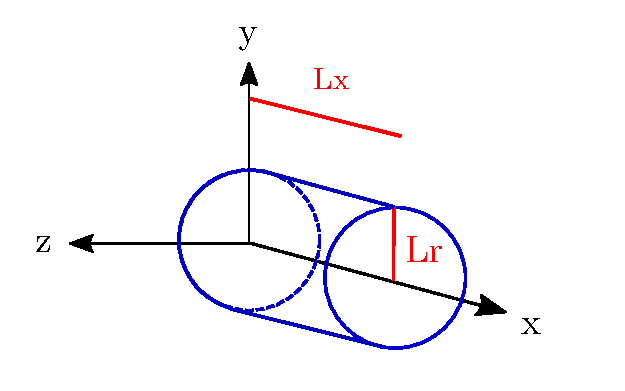
\includegraphics[width=1\linewidth]{Reference.pdf}
     \caption{Reference axes of the simulation. The simulation window corresponds to the cylinder with radius \commandline{Lr} and length \commandline{Lx}. }\label{reference_axes}
   \end{minipage}\hfill
   \begin{minipage}{0.65\textwidth}
     \centering
     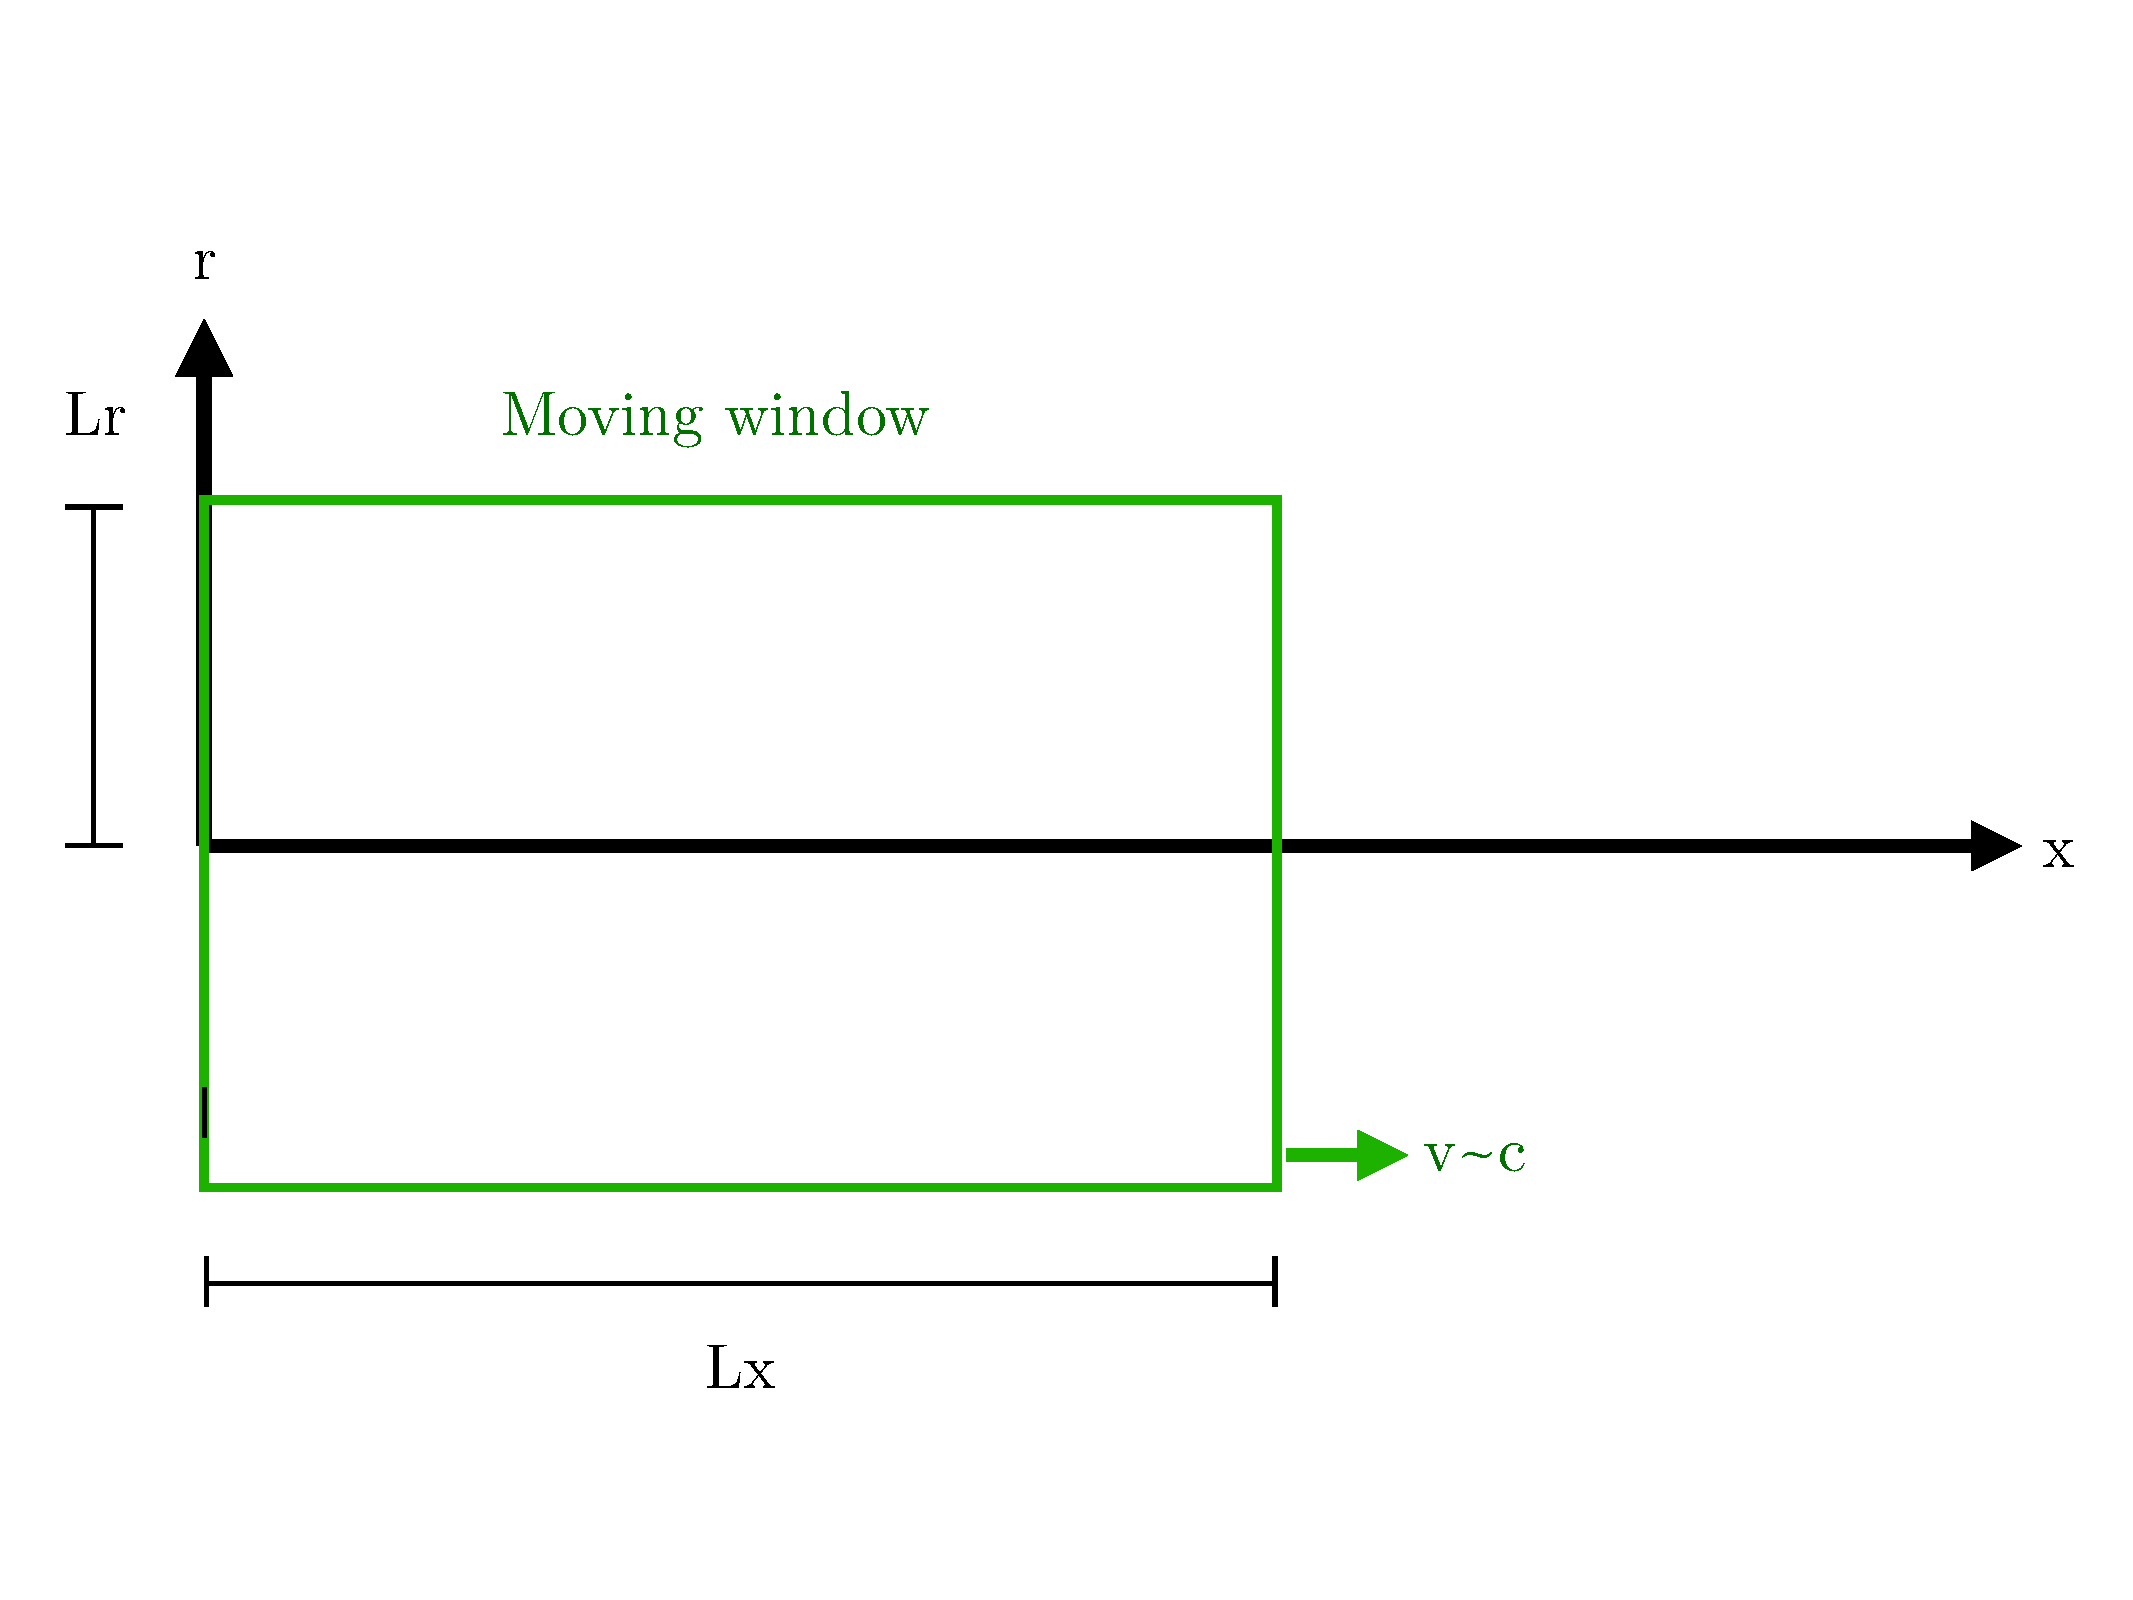
\includegraphics[width=1\linewidth]{Schema_Simulation_0.pdf}
     \caption{Simulation Setup in this Section (not in scale).}\label{Schema0}
   \end{minipage}
\end{figure}

\subsection*{The \commandline{MovingWindow} block}
Note a block called \commandline{MovingWindow} in the input namelist. In the considered physical case,  a laser pulse with duration of the order of tens femtoseconds propagating for $\approx 400$ $\mu$m along the positive $x$ direction is simulated. We are interested only in phenomena near the laser pulse (within tens of microns) like plasma wave excitation, so it would be very inefficient to simulate all the physical space (and plasma particles when present) in a box with length of hundreds of microns. For this reason, the code has the option to use a \emph{Moving} \emph{Window}, i.e. like having a camera moving at the speed we want  along the positive $x$ direction. In this physical case, it is convenient to have a window/camera moving with the laser, so we will set the average speed of the moving window to $c$ to follow the laser. For this reason, you will see the laser pulse almost immobile in your simulation window. The size of the our moving simulation window will be of tens of microns, so if it moves with the laser we will be sure to see all the relevant phenomena of plasma wave excitation near the pulse.

\subsection*{The \commandline{Diag} blocks}
At the end of the namelist there are blocks starting with the word \commandline{Diag}. As you can imagine, they are the diagnostic of the code, our interface with the simulation results. The first \commandline{Diag} is a \commandline{DiagProbe} defined on a line (so a 1D diagnostic), on the propagation axis of the laser (the $x$ axis). This diagnostic will show in output the value of some physical fields along that axis. We call this probe \commandline{Probe0} (the 0 because it is the first \commandline{Probe} in the namelist). The second diagnostic block is a \commandline{DiagProbe} defined on the plane $xy$ (so a 2D diagnostic). This is the second probe of the namelist, so it is called \commandline{Probe1}. Inside these \commandline{DiagProbe} blocks, the physical quantities in output we are interested in are specified. For this practical, you don't have to write new postprocessing scripts, since \smilei includes a postprocessing library, called \commandline{happi}, to analyze the code results. For the purposes of the practical, the \commandline{happi} commands explained in Appendix \ref{happi} and the postprocessing scripts you will be given are sufficient to start. However, if you prefer to work with \commandline{numpy} arrays in Python, at the end of Appendix \ref{happi} you will find also how to export the output to that format. If you prefer to work with other languages for postprocessing, you can export the data to a \commandline{numpy} array and then write them to a file readable with your language of choice.
The last exercises of this practical will ask to write postprocessing scripts, using the commands you will find in the already provided postprocessing scripts.

\section{Simulation Exercises}
After the preliminary steps described in the Introduction (including the first two exercises), you should be ready to proceed with tha practical exercises.  We will arrive to the simulations of plasma acceleration in three steps:
\begin{itemize}
\item simulation of the laser pulse propagating in vacuum;
\item simulation of the plasma waves in the wake of the laser pulse;
\item simulation of the acceleration of electrons in the laser wake wave
\end{itemize}

Initially the input namelist only has the essential blocks (e.g.  the Main block),  the other blocks are commented. The mentioned three steps will be completed progressively decommenting the laser pulse block, the plasma electron block and the blocks used for the electron bunch.

To complete the practical, read the instructions of the following sections, complete the related simulation exercises and ask the instructor in case of doubts. 

Without further ado, let's get started!

\subsection{Laser pulse in vacuum}
Everything is ready to run your first simulation: just uncomment the lines with the laser pulse parameters and the \commandline{LaserEnvelopeGaussian} block. This block defines a Gaussian laser pulse in the simulation. The considered pulse will also have a Gaussian temporal envelope profile.

Normally you would simulate a laser pulse with all the high frequency oscillations at frequency $\omega_0=2\pi c/\lambda_0$. This is surely the most accurate approach, but it would need a very fine resolution and integration timestep and consequently a very long simulation time (see Fig. \ref{fig:envelope}). Note that in the most simple laser wakefield acceleration set-ups the laser pulse temporal envelope (often modeled with a Gaussian profile) will contain many optical oscillations.


\begin{figure}[!htb]
   \begin{minipage}{0.35\textwidth}
     \centering
     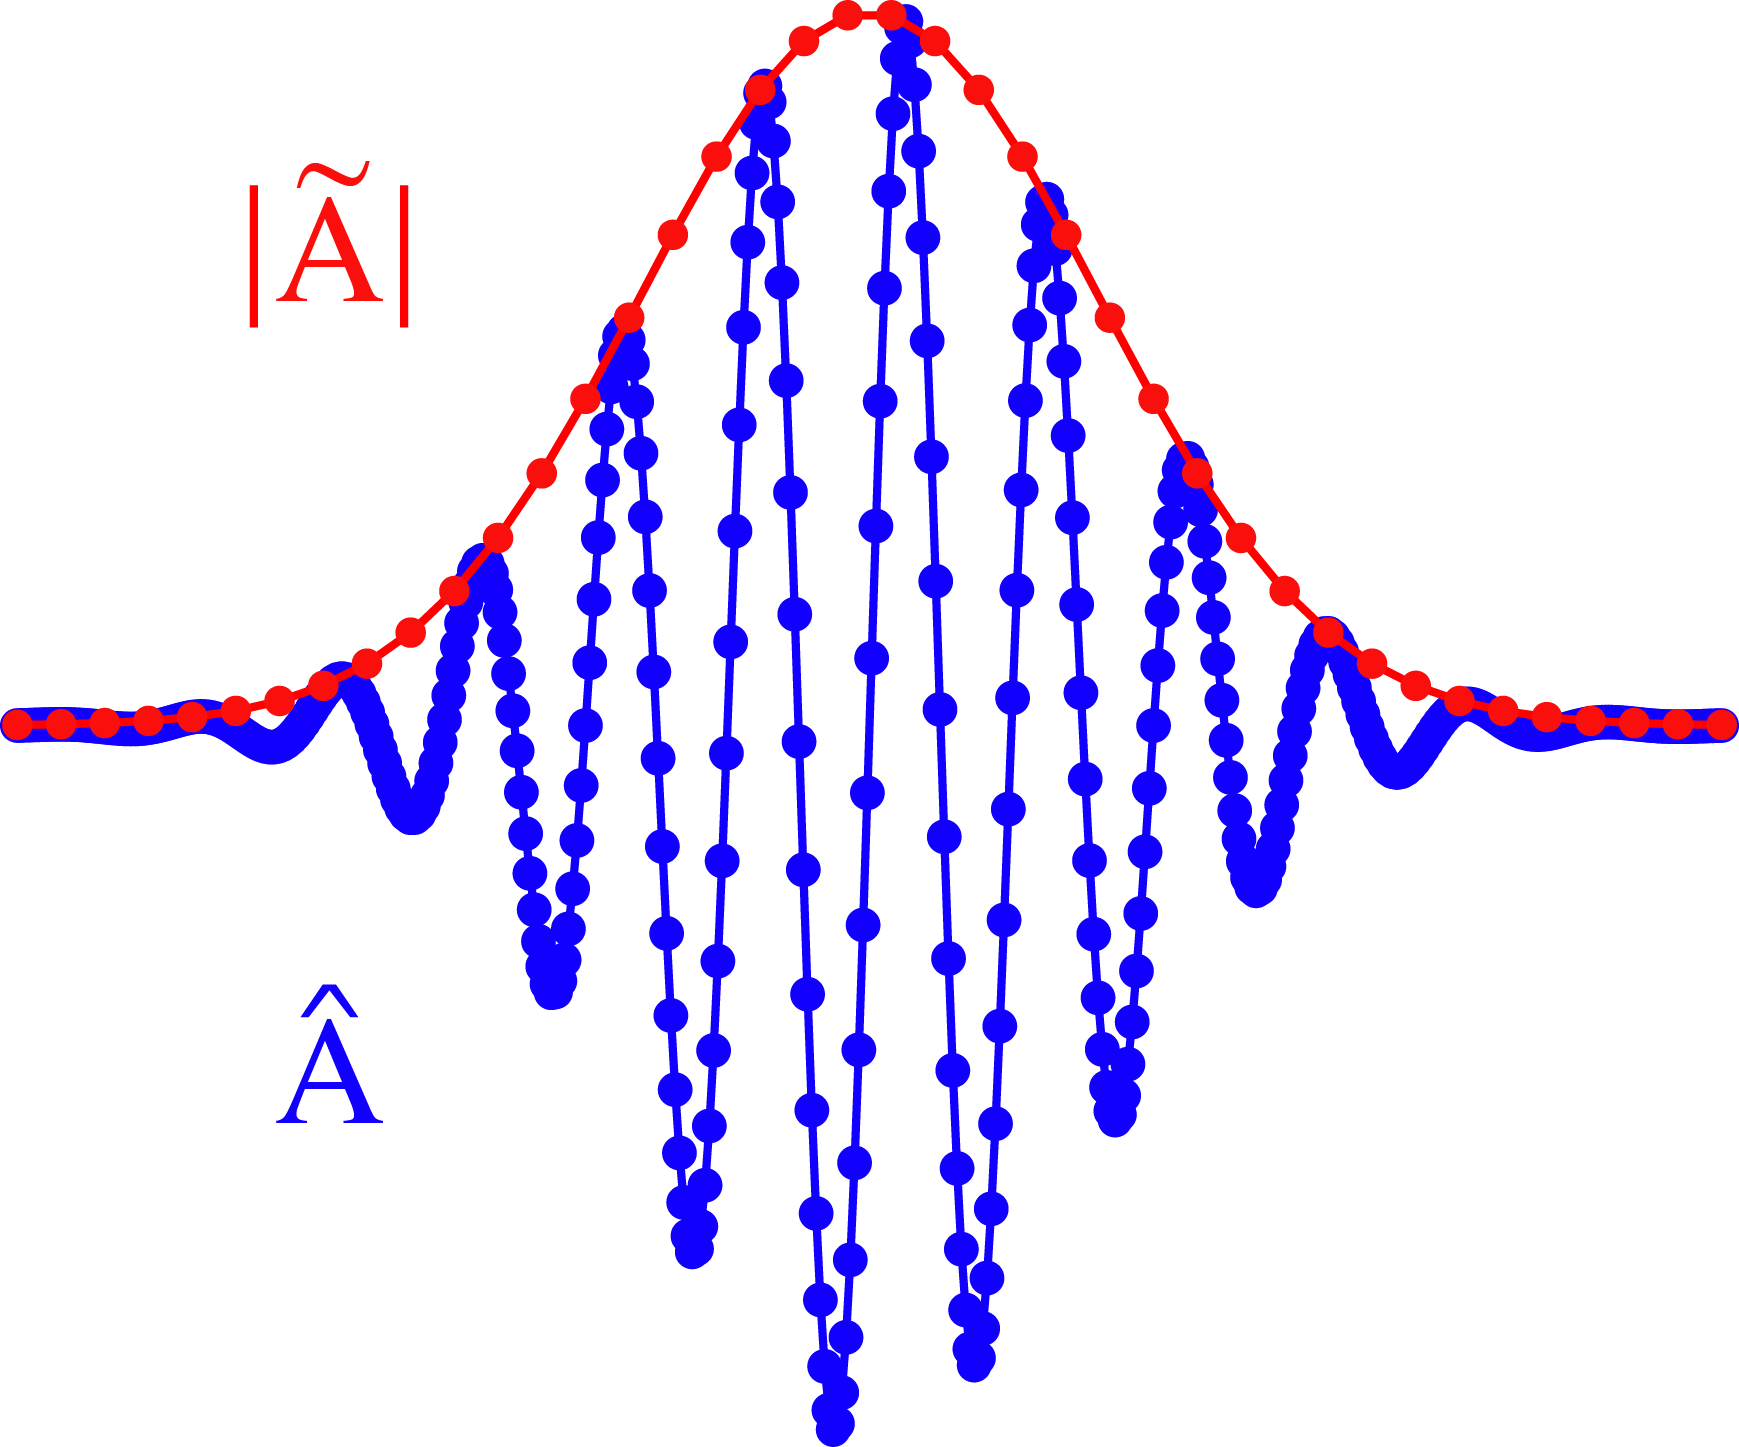
\includegraphics[width=1\linewidth]{Envelope_Figure.png}
     \caption{Blue line: vector potential $\hat{A}$ of a laser pulse with Gaussian envelope. Red line: its absolute value $|\tilde{A}|$.  Both lines are sampled by a suitable number of points. Note that much less points are necessary to sample the envelope.}\label{fig:envelope}
   \end{minipage}\hfill
   \begin{minipage}{0.65\textwidth}
     \centering
     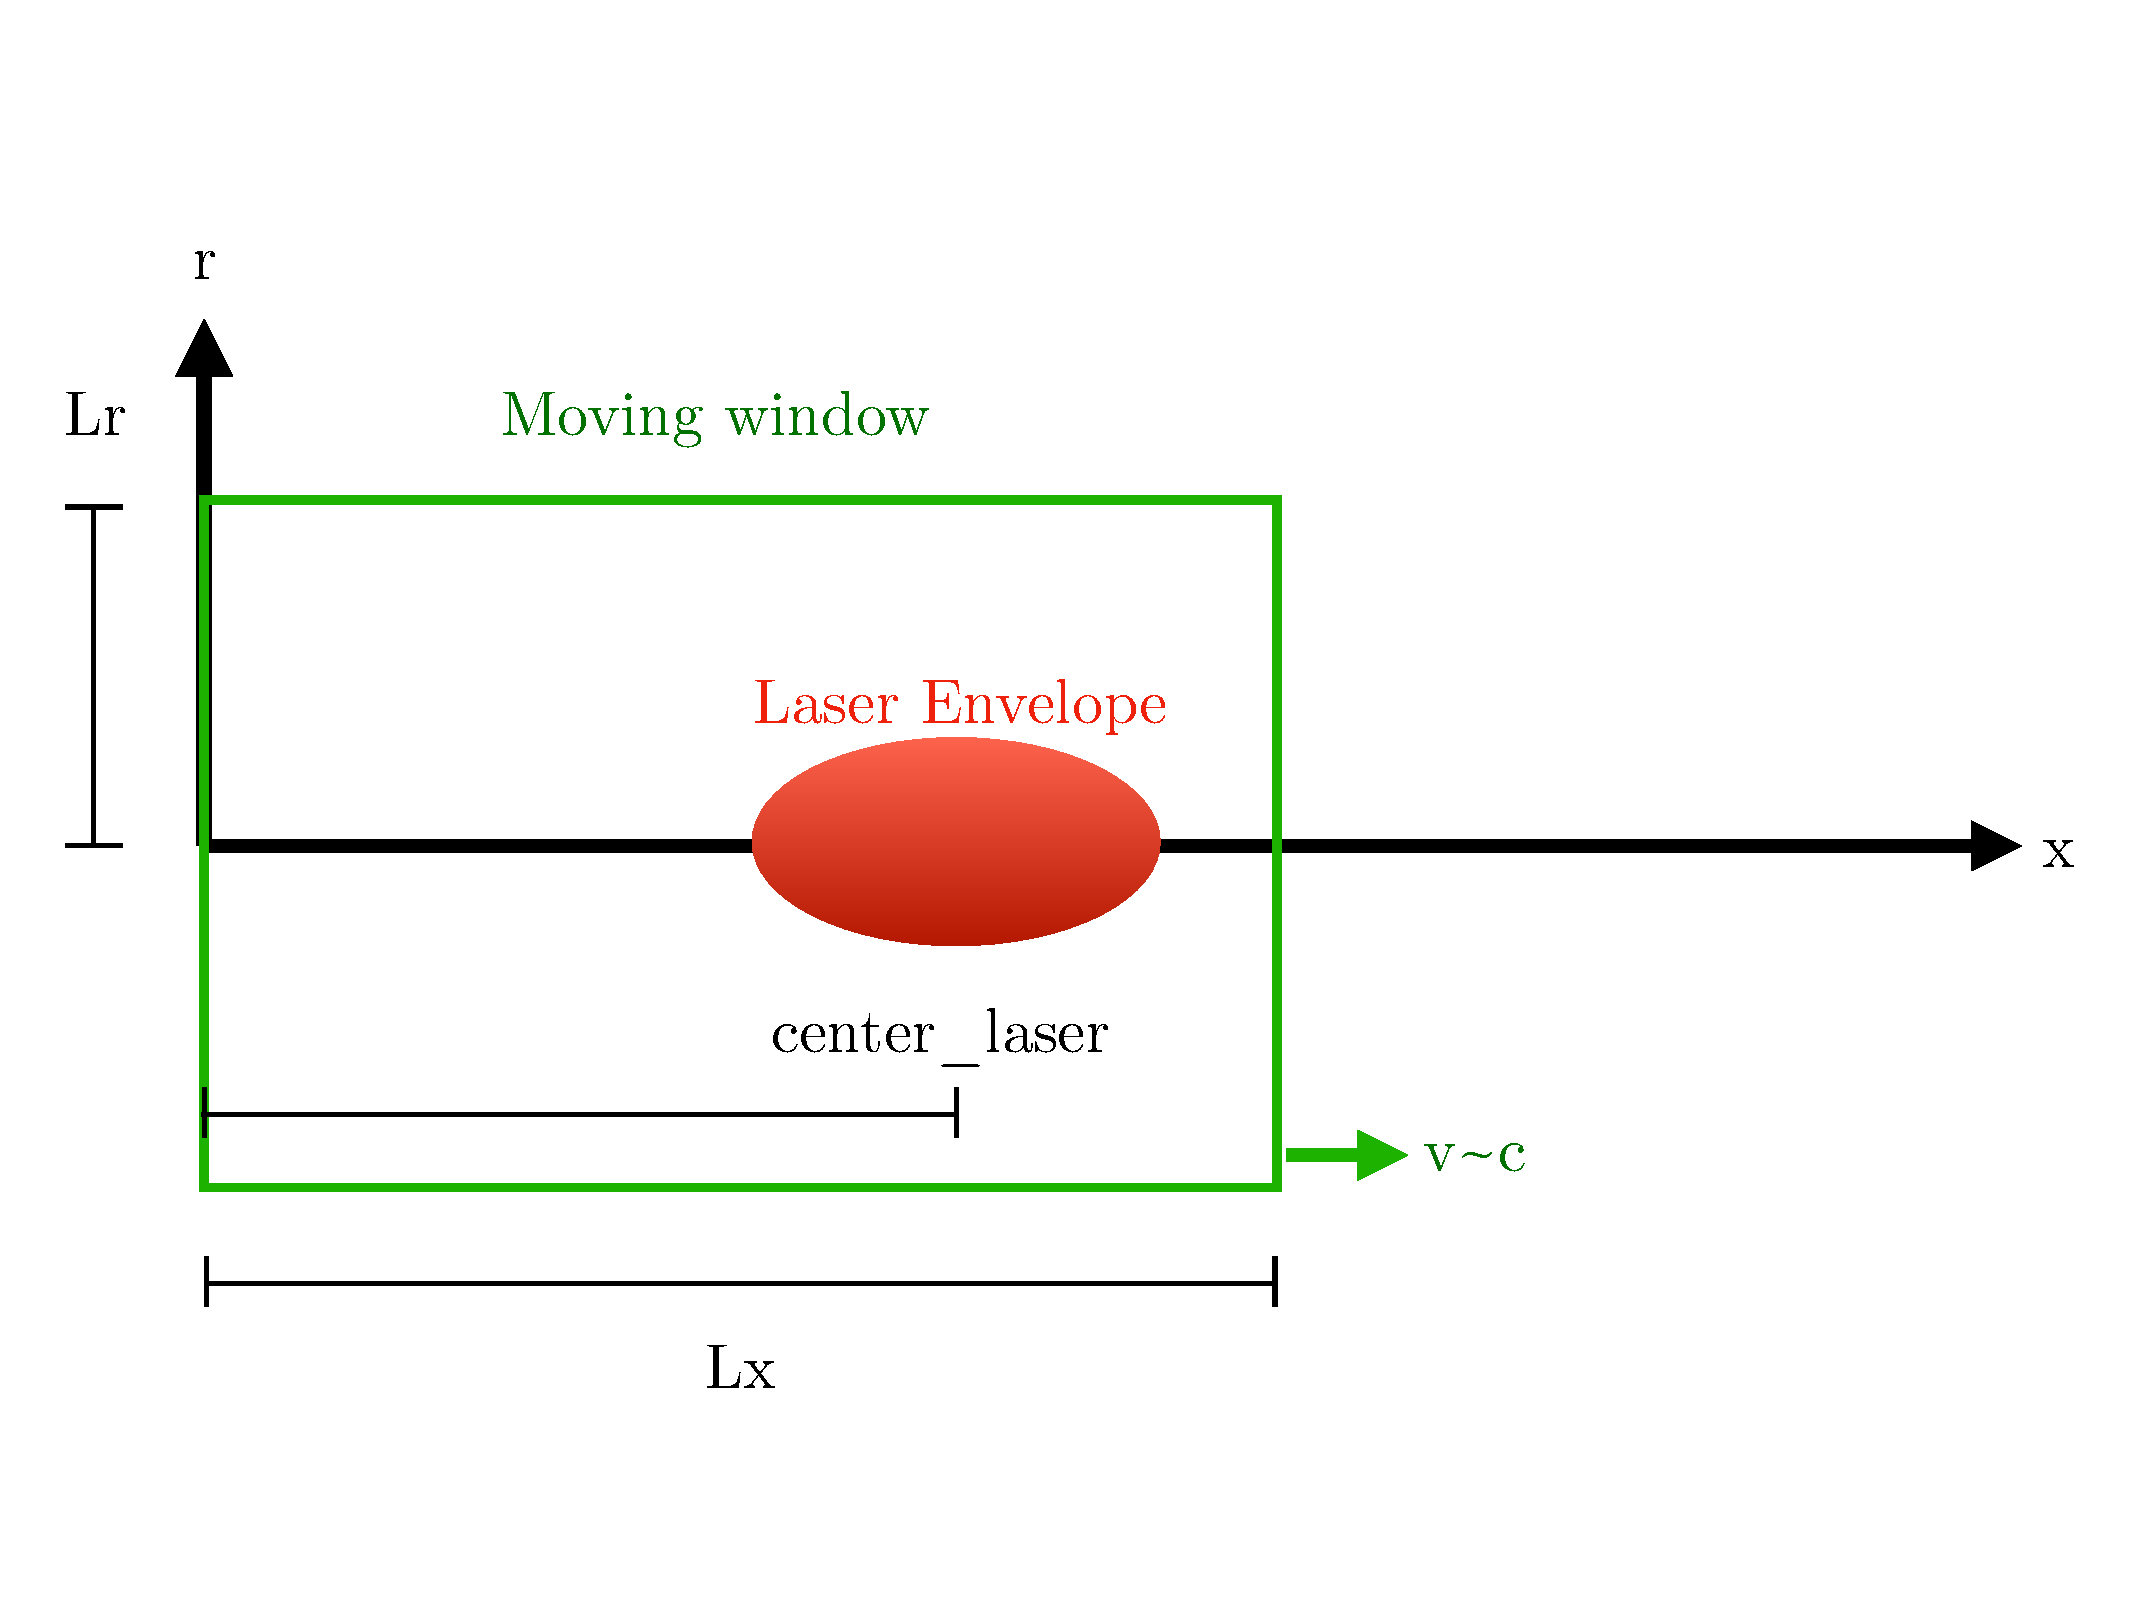
\includegraphics[width=1\linewidth]{Schema_Simulation_1.pdf}
     \caption{Simulation Setup in this Section (not in scale).}\label{Schema1}
   \end{minipage}
\end{figure}

Thus, using a laser envelope model it will be possible to describe the laser and its interaction with the plasma only in terms of its envelope and have quick simulations (due to the coarser sampling). In this kind of model, the laser evolution is described by an envelope equation (like in a paraxial wave equation for example). The laser radiation pressure on the plasma particles is described by the ponderomotive force (which depends only on the laser pulse envelope). With this approach, the accuracy of the results will be enough to explore the basic physics of laser plasma acceleration and at the same time you will be able to perform quicker simulations. \\

\textbf{ Note:} since an envelope model is used for the laser,  the electromagnetic fields in output like \commandline{Ex},\commandline{Ey} (and the densities like \commandline{Rho}) will only show the average of these quantities over the optical oscillations of the laser and not including the laser field. Thus, these quantities will not show the oscillations at $\omega_0$ and $2\omega_0$ normally seen in a simulation of LWFA without an envelope model. The electromagnetic fields in output will be those generated in the plasma, while the absolute value of the envelope of the transverse electric field of the laser is contained in the quantity \commandline{Env\_E\_abs}. \\

The simulation now includes a moving window and a laser pulse, modeled with its envelope, as in Fig. \ref{Schema1}.\\

\textbf{ - Exercise 3:} What are the waist size, FWHM duration in field and intensity of the laser pulse specified in the namelist? Where is the laser pulse center placed in the simulation window at the start of the simulation? Where is the focal plane of the laser?\\

\textbf{ - Exercise 4:} The normalized laser peak field is given by $a_0=\frac{eE}{m_e\omega_0 c}$, where $E$ is the peak laser electric field and $\omega_0=2\pi c/\lambda_0$ is the laser central frequency ($\lambda_0=0.8$ $\mu m$.) What is the peak intensity $I=\frac{c\epsilon_0}{2}|E|^2$ of the laser pulse? Suggestion: the input namelist contains the physical quantities that you may need for the conversions.\\

After you have uncommented the necessary lines (try again \commandline{./smilei\_test Inputnamelist.py}), launch the simulation.  When the simulation is completed, open \commandline{IPython} with the command \commandline{ipython}. Then, you can check the initial position of the laser through the commands:\\

\commandline{import happi; S =  happi.Open("path/to/simulation")}

\commandline{S.Probe.Probe0("Env\_E\_abs",timesteps=0).plot( figure=1 )}

\commandline{S.Probe.Probe1("Env\_E\_abs",timesteps=0).plot( figure=2 )}\\

\commandline{Probe0} is a 1D diagnostic defined on the laser propagation axis, while \commandline{Probe1} is a 2D diagnostic defined on the plane $xy$.  Note that in the commands we have specified \commandline{timesteps=0} to see the laser pulse at the start of the simulation. Check that the initial laser position that you are seeing is the same specified in the input namelist. Remember that the laser pulse is modeled through its envelope, so you won't see its high frequency oscillations with wavelength $\lambda_0$.\\

Let's study the laser diffraction in vacuum. To see the evolution of the laser, use:\\ 

\commandline{S.Probe.Probe1("Env\_E\_abs").animate( figure=3 )}\\

Note that the use of the \commandline{Moving Window} will make the laser seem immobile in the simulation, but it is actually moving at speed $c$ and the \commandline{Moving Window} is following it with the same speed.

If you don't specify a \commandline{vmax} value (the colorbar maximum) in the previous animation command, \commandline{happi} will change it at each iteration. To better see the laser diffraction, try to  specify \commandline{vmax=0.05} in the previous command, or use \commandline{.slide()} instead of \commandline{.animate()}. For example:\\

\commandline{S.Probe.Probe1("Env\_E\_abs").slide( figure=3,vmax=0.05 )}\\

\textbf{ - Exercise  5:} Let's check that the Gaussian laser pulse diffracts following the theory for a Gaussian beam: $w(x)=w_0\sqrt{1+x^2/x_R^2}$, where $w_0$ is the initial laser waist size, $w(x)$ the laser waist size at propagation distance $x$, $x_R$ is the Rayleigh length $x_R=\pi w_0^2/\lambda_0$. 

What is the theoretical Rayleigh length $x_R$ ?\\

\textbf{ - Exercise  6:} Use the script \commandline{Laser\_waist\_theory\_vs\_Smilei.py} to compare the analytical diffraction law of the previous exercise and the code results. Copy the script in the simulation folder or call the script from that folder. The script loads the results, then loops over the iterations available in output and computes the laser pulse waist $w(x)$ as 
\begin{equation}
w(x)=2\times\frac{\int\int|\tilde{A}|^2  (y-\bar{y})^2 dx dy}{\int\int |\tilde{A}|^2  dx dy}.
\end{equation} Since the laser field goes to zero at the borders of the simulation window, instead of integrating over the infinite extension of space we can limit our integrals to the simulation window space. After this computation, the simulated waist is compared to the corresponding analytical value. Run the script (from \commandline{IPython} use \commandline{\%run Laser\_waist\_theory\_vs\_Smilei.py} ) to plot the comparison.

\subsection{Plasma waves}

\subsubsection{Linear plasma waves}
In the previous section it was verified that the laser pulse behaves as expected in vacuum. Now, let's add a preionized hydrogen plasma to excite plasma waves.
The laser will be intense enough to assume the gas was already ionized much before the arrival of the laser pulse peak (see the laser intensity computed in \textbf{Exercise 3}).

Uncomment the first \commandline{Species} block, the related variable definitions and take some time to read them carefully. This block defines a particle \commandline{Species} in the simulation, whose name is \commandline{plasmaelectrons}. Note the normalized mass and normalized charge of these particles defined in this block (\commandline{1.0}. and \commandline{-1.0}. respectively). Since the normalizing mass and charge are the electron mass and the unit charge (see Table \ref{tab_normalisations}) we know that these particles are electrons.

Since the simulation is in cylindrical coordinates, the plasma electron density profile in general will be defined at coordinates $(x,r)$, where $r$ is the distance from the laser propagation axis. As you can see, for each point in space $(x,r)$ the plasma density profile is defined by the function \commandline{plasma\_density$(x,r)$}. After a short linear ramp, this plasma density profile is uniform in a region confined to a distance \commandline{Radius\_plasma=$22$ $\mu$m} from the laser propagation axis. This of course is not a realistic size for a real-world plasma for plasma acceleration. However we can simulate a small-scale plasma like this without significantly changing the results, since the phenomena of interest occur near the laser pulse. Including particles far from the laser propagation axis would increase the computation time without changing the results. You can check it at the end of the practical increasing the plasma transverse size, bear in mind that this will increase the simulation time.\\

The simulation now includes a moving window, a laser pulse (modeled with its envelope) and plasma electrons, as in Fig. \ref{Schema2}.

\begin{figure}[h!]
  \begin{center}
  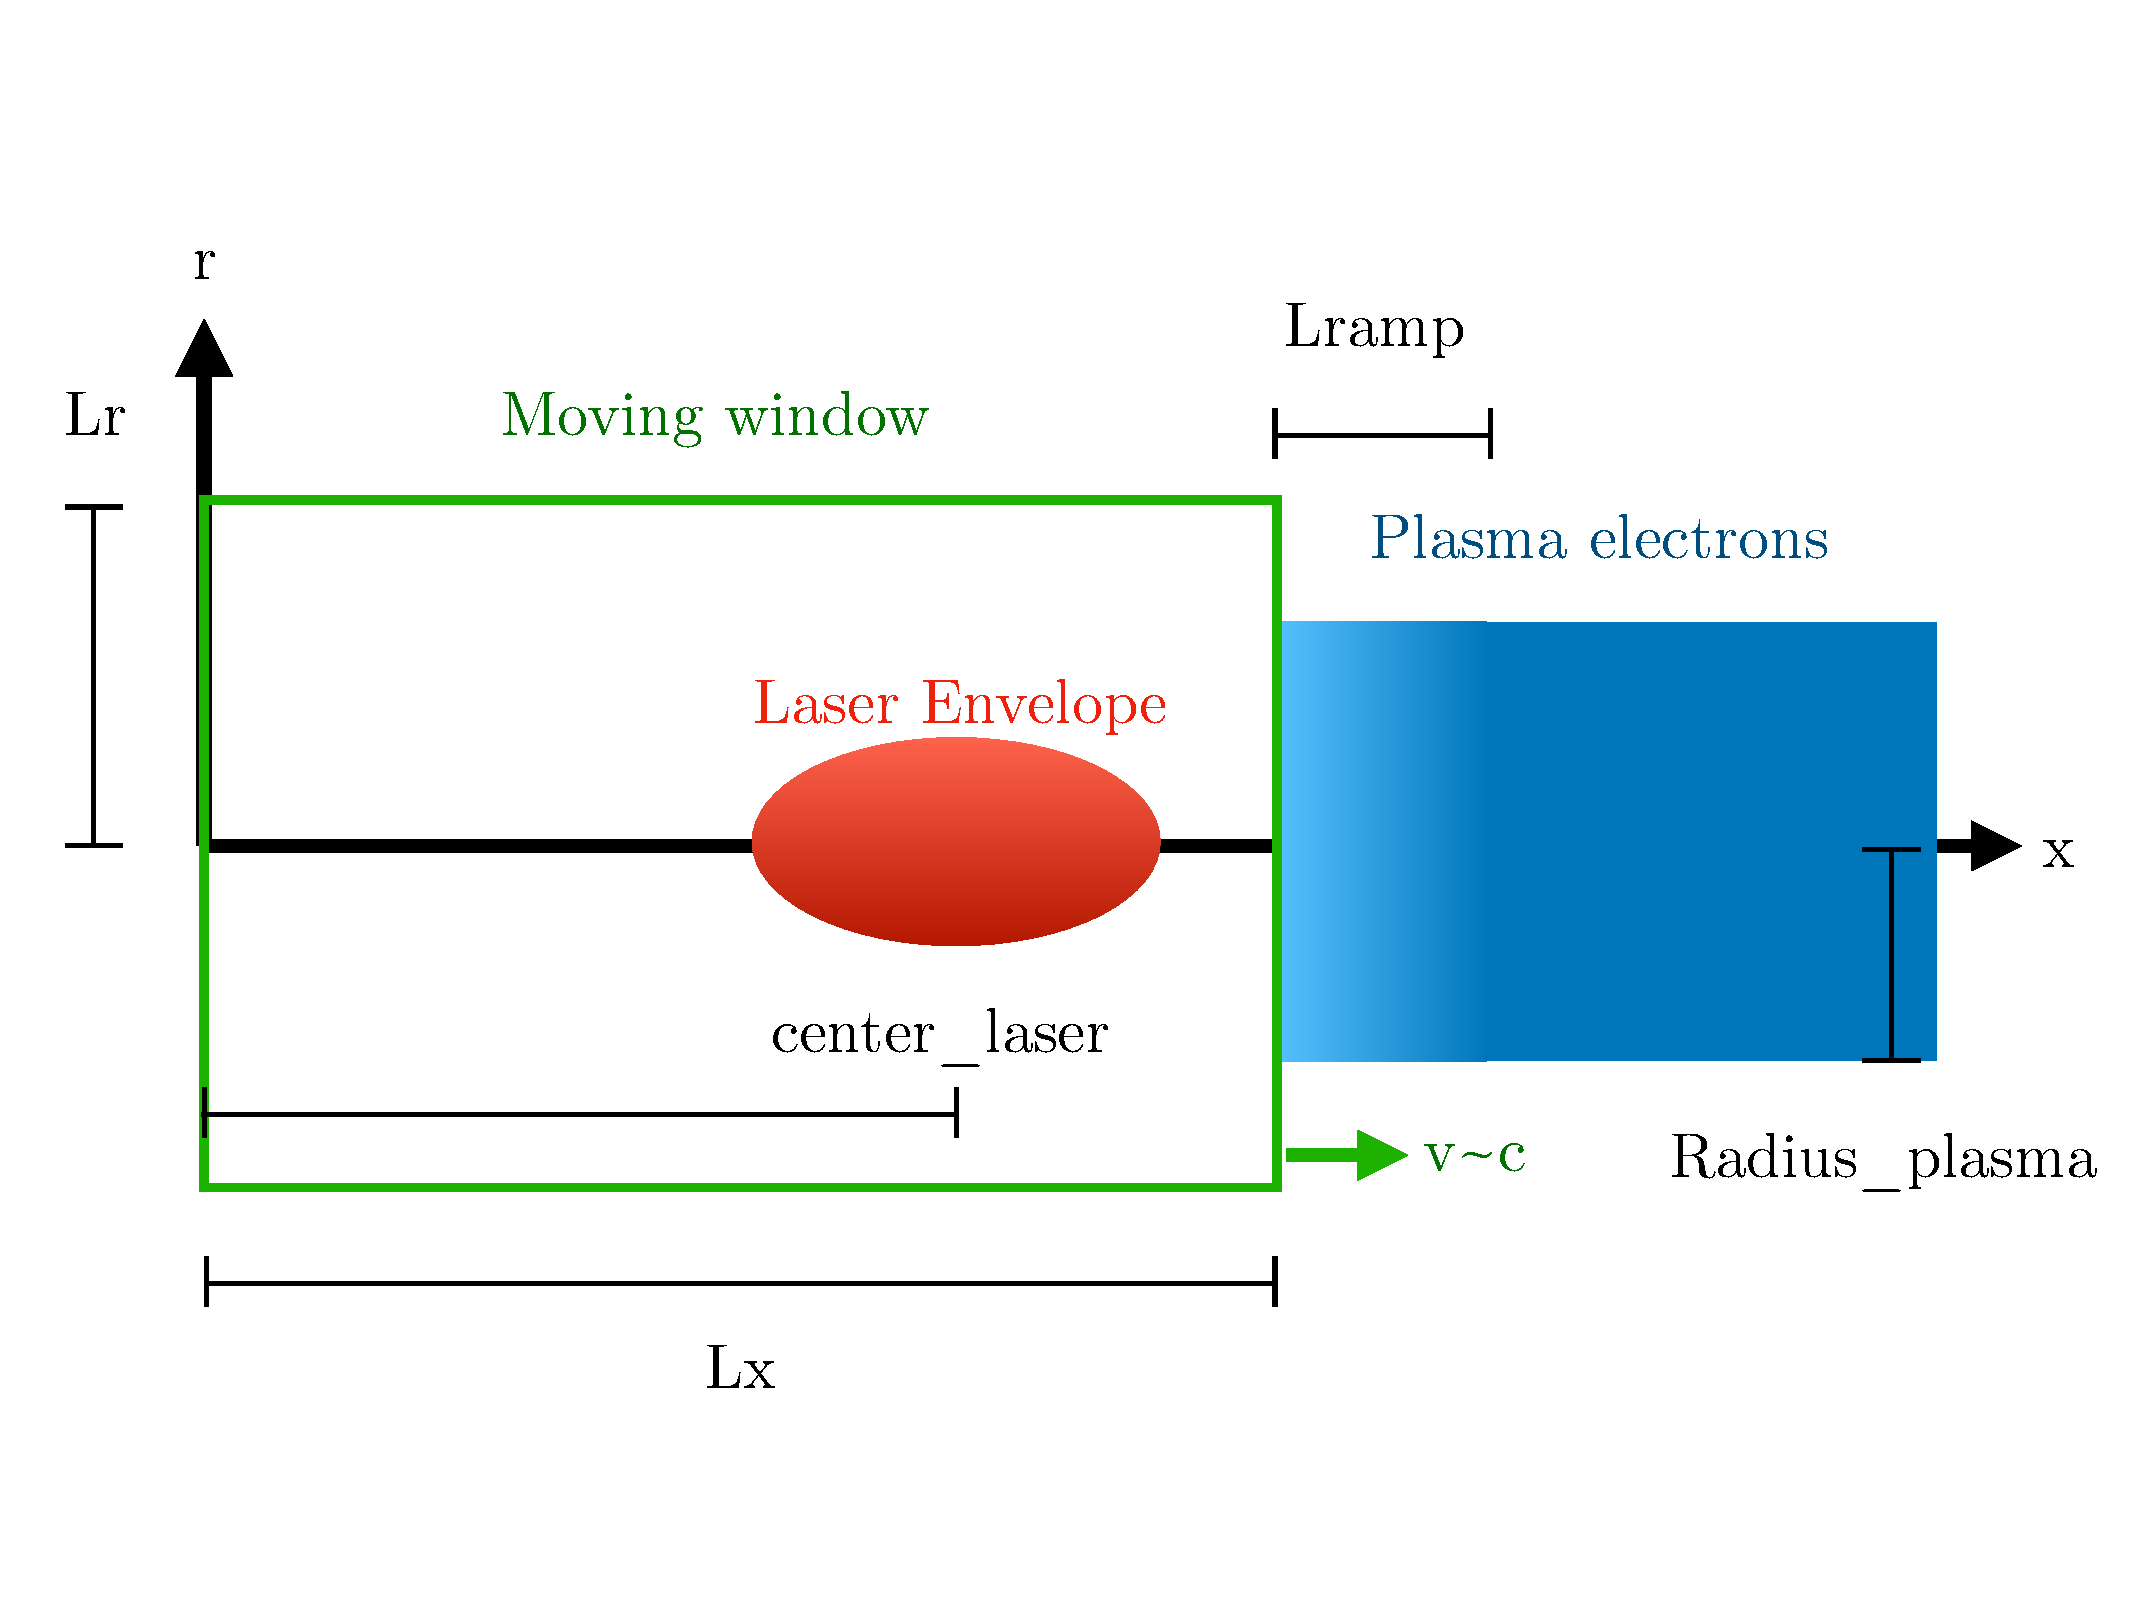
\includegraphics[scale=0.3]{Schema_Simulation_2.pdf}
  \end{center}
  \caption{Simulation Setup in this Section (not in scale) at $t=0$.}
  \label{Schema2}
\end{figure}

As we did with the simulation of the laser pulse diffraction in vacuum,  the first step will be to verify that the plasma behaves as predicted by the analytical theory. If we reduce the laser pulse $a_0$ to $0.01$, the laser pulse will satisfy the conditions for the applicability of the 1D linear theory of plasma wave excitation. The  analytical 1D linear theory predicts the formation of a sinusoidal wave at plasma frequency $\omega_p=\sqrt{e^2n_0/m_e\epsilon_0}$ behind the laser, where $n_0$ is the plasma density.\\

\textbf{ - Exercise 7:} As you can see, the plasma density has a value $n_0=0.0008$ (in normalized units, i.e.  normalized by the critical density in this case) in the uniform region.  What is its value in physical units (electrons/cm$^{-3}$)? \textit{Hint:} see Table \ref{tab_normalisations} in Section \ref{units}. If you wanted to specify $n_0$ from SI units to code units using the conversion with the variable \commandline{ncrit} in the namelist, what command should you use? You don't have to change the namelist. \\

\textbf{ - Exercise 8:} Launch the simulation with $a_0=0.01$. Study the evolution of the electric field \commandline{Ex} with \commandline{Probe0} and \commandline{Probe1} (same plot commands of the previous section, but applied to \commandline{Ex}). What is the theoretical plasma wavelength $\lambda_p=2\pi c/\omega_p$? What is the plasma wavelength inferred from the simulation results?\\


\textbf{ - Exercise 9:} The longitudinal electric field on the axis of this linear plasma wave, according to the 1D linear theory, is given by (in physical units):
\begin{equation}\label{linear_theory}
E_x(x) = \frac{m_e c^2}{e}\frac{k_p^2}{4} \int_x^{+\infty} |\tilde{A}|^2\rm{cos}\left[\omega_p(x-x')\right]dx'.\\
\end{equation}
Use the script \commandline{Ex\_linear\_theory\_vs\_Smilei.py} to compare the analytical result given by Eq. \ref{linear_theory} and the simulated results (\commandline{\%run Ex\_linear\_theory\_vs\_Smilei.py} on \commandline{IPython}). Again, you will need to copy the script in the simulation folder or to call it from there. The script reads the absolute value of the envelope of the laser $|\tilde{A}|$ from the simulation at a given time and then implements Eq. \ref{linear_theory} to compute the analytical result for $E_x$. Then it reads the longitudinal electric field \commandline{Ex} of the simulation to compare the theory with the simulation results. Does the simulation agree with theory?

\subsubsection {Nonlinear plasma waves}
With the laser and plasma parameters in the namelist, for $a_0\ll1$ the excited plasma waves will be in the linear regime. As we saw in the previous exercise, the plasma wave in the wake of  the laser is sinusoidal in this regime.
Increasing $a_0$, the laser will be more intense and when $a_0\gtrsim1$ the plasma electrons will start to  be pushed to relativistic velocities. Their relativistically increased inertia will elongate the plasma period and plasma wavelength, and electron accumulation will occur at the end of each wave period. Increasing $a_0$, the longitudinal electric field waveform will change from a sinusoid to a sawtooth wave. In this regime of interest for plasma acceleration PIC simulations become necessary, because for this regime there are no general analytical solutions to the coupled Vlasov-Maxwell system of equations,  and fluid theory cannot be applied.\\

Create three folders, \commandline{sim1}, \commandline{sim2}, \commandline{sim3}, where you will launch the simulation  with $a_0=0.5,\thinspace 1.4,\thinspace 2.0$ respectively. Take a look to the longitudinal electric field on axis (\commandline{Probe0}) and to the 2D plasma density (\commandline{Probe1}):\\

\commandline{S.Probe.Probe0("Ex").animate( figure=1 )}

\commandline{S.Probe.Probe1("-Rho").animate( figure=2 )}\\

In the linear case probably you will not be able to see easily the oscillations in the density, but they can be easily seen in the electric field $E_x$. In the nonlinear cases (higher $a_0$) you will need to lower the \commandline{vmax} in the plot/animate command to see the formation of  the wake. This because at the end of the plasma wave period there is an accumulation of electrons, which hides the other values of the charge density if \commandline{vmax}  is not properly chosen.
As you can see, increasing the $a_0$, the nonlinearities of wake excitation will be progressively more evident. For each simulation, take a look to the excitation of the wave with the command \commandline{animate} of \commandline{happi}.\\

\textbf{ - Exercise 10:} It is interesting to compare the longitudinal electric field of these three simulations to see how the wave changes increasing $a_0$. With \commandline{happi} (or Python if you prefer) you can easily do it. Here are the commands for \commandline{happi}:\\

\commandline{import happi}

\small{\commandline{S1 = happi.Open("path/to/sim1"); Ex1 = S1.Probe.Probe0("Ex",timesteps=1000,label="a0 = 0.5")}}

\commandline{S2 = happi.Open("path/to/sim2"); Ex2 = S2.Probe.Probe0("Ex",timesteps=1000,label="a0 = 1.4")}

\commandline{S3 = happi.Open("path/to/sim3"); Ex3 = S3.Probe.Probe0("Ex",timesteps=1000,label="a0 = 2.0")}

\commandline{happi.multiPlot(Ex1,Ex2,Ex3,figure=3)}\\

The last command, \commandline{multiPlot}, is used to superpose multiple lines in the same plot window.  This command will be used also in some of the exercises of the following section.



\subsubsection*{Behind the curtain: why ions are not present? (Optional)} A plasma for laser wakefield acceleration is normally made of ions and electrons at least, so why ions are not present in this namelist? The answer can be found in the properties of Maxwell's Equations and implies some derivations.  For the moment it is sufficient to say that, since we set to zero the plasma electromagnetic field at the beginning of these simulations, and that we solve carefully Maxwell's Equations and the particles equations of motion, defining the plasma electrons will make the code behave as if there was also a neutralizing layer of immobile ions. Since ions do not move in the timescales of interest for the phenomena we are simulating (their mass is at  least $2000$ times larger than the electron mass), this is a reasonable approximation that in addition removes the need to simulate also the ions, with a significant computational gain. The complete answer for the interested reader can be found in the dedicated section of this tutorial \url{https://smileipic.github.io/tutorials/advanced_wakefield_electron_beam.html}.

\subsection{Laser plasma acceleration with external injection}
Finally everything is ready to simulate a plasma accelerator. As a surfer rides the waves in the ocean,  under some conditions a bunch of electrons can be accelerated by plasma waves. Remember that an immobile surfer will not be accelerated by a wave. To efficiently interact with the wave, the surfer must first pad to acquire some velocity. If the surfer moves near to the speed of the wave, he will see an accelerating phase of the wave for all the interaction.
Following the same analogy,  the electrons to be accelerated must be injected in the accelerated phase of the plasma wave, with a speed near the wave velocity  ($\approx c$). Many clever injection schemes have been investigated since  the years 2000s, where the electrons of the plasma itself are someway injected in the laser-driven wave. However, although it is more experimentally difficult to realize, in this practical external injection will be studied, i.e. the injection of a relativistic electron beam from outside the plasma. This will allow to understand the basic concepts of electron injection in a plasma wave. \\

Set again the $a_0$ of the laser to  the value $1.8$ . Uncomment the second \commandline{Species} block, the related variable definitions and take some time to read them carefully. As you can see, this block defines a \commandline{Species} called \commandline{electronbunch}, which we will inject in the plasma wave for acceleration. As for the \commandline{Species} called \commandline{plasmaelectrons} of the previous  Sections, these particles have normalized \commandline{charge} and \commandline{mass} equal to \commandline{-1.0} and \commandline{1.0} respectively, thus they are electrons. In this case,  the number density will not be defined through a density profile function, but the charge, the coordinates and the momenta of each of the bunch's macro-particles will be given to the code through arrays. The variable \commandline{npart} defines the number of macro-particles (in  this case 20000) of the bunch, and this will be also the length of the bunch arrays: to initialize \commandline{npart} particles one by one, you need an array of length \commandline{npart} for their $x$ coordinates, an array of length \commandline{npart} for their $y$ coordinates and for the $z$ coordinates. These coordinates will be stored in the variable called \commandline{array\_position}, which keeps also an array of length \commandline{npart} to store the charge of each macro-particle (you don't need to understand right now how it is defined). You will need also need to initialize similarly the momenta of the particle, which are stored similarly in the variable \commandline{array\_momentum}. In this case, these coordinates and momenta are generated from a Gaussian pseudorandom distribution, multiplying the numbers by their standard deviations to have a bunch with a rms size, rms momentum spread and rms energy spread that we want. You will note that the initialized bunch is already relativistic and has a Gaussian distribution in all the coordinate-momenta subplanes in the phase space.\\

For your future  simulation work, this initialization method can be used also to use a particle distribution obtained from another code (a magnetic transport code for conventional accelerators for example). Instead of generating randomly the particles coordinates and momenta, you only need to read them with Python. The arrays you will obtain can thus be directly used by \smilei. Note that you can do this also for a plasma density distribution or laser intensity profile that you measure in an experiment. Instead of defining them through a Python function, you  can read the experimental data and feed them to \smilei to simulate your measured plasma and/or laser profile.\\

The simulation now includes a moving window, a laser pulse (modeled with its envelope), plasma electrons and an electron bunch, as in Fig. \ref{Schema3}.\\

\begin{figure}[h!]
  \begin{center}
  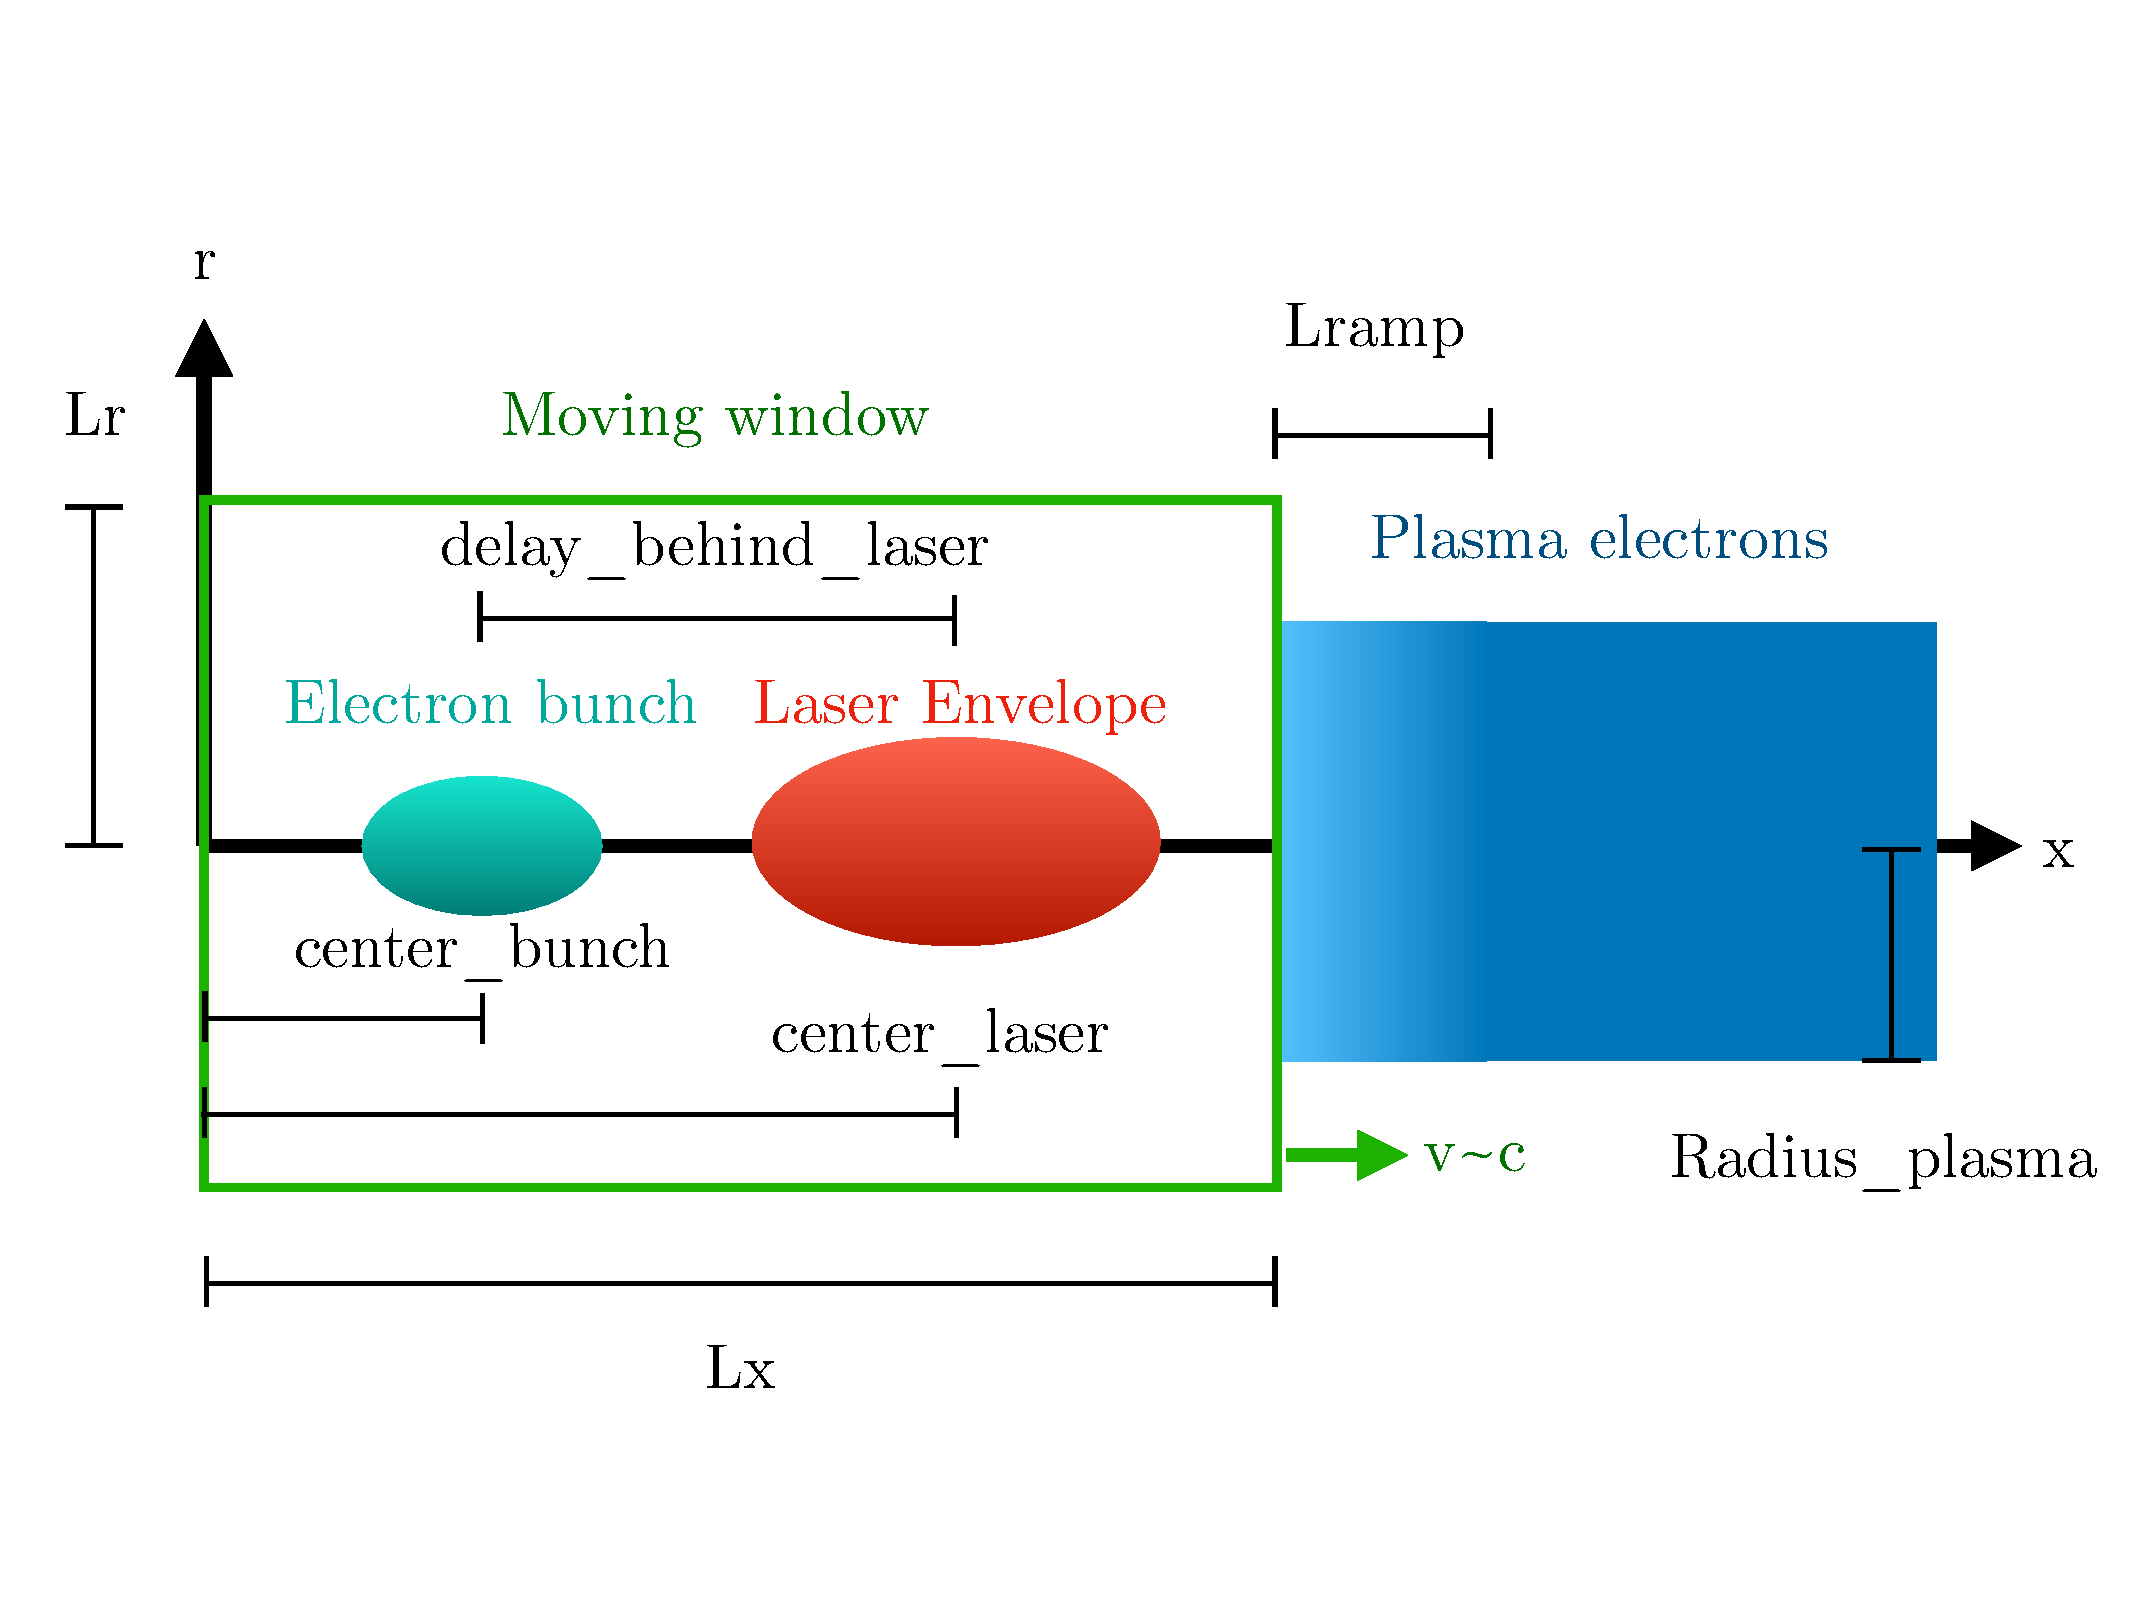
\includegraphics[scale=0.3]{Schema_Simulation_3.pdf}
  \end{center}
  \caption{Simulation Setup in this Section (not in scale).}
  \label{Schema3}
\end{figure}

\textbf{ - Exercise 11:} Reading the namelist, provide a description of the electron bunch at $t=0$: total charge, energy, rms sizes along $x$, $y$, $z$, rms energy spread, emittance  along the transverse planes. Where is the electron bunch placed in the window initially? \\

\subsection*{The \commandline{DiagTrackParticles} block}
To have a close look to the electron bunch during its propagation,  you will need to uncomment also the \commandline{DiagTrackParticles} block. As the name suggests, this diagnostic block allows to track particles, specified by their species name and some filter. Using a filter (e.g. selecting only the particles with energy higher than $50$ MeV) is particularly useful when you have many particles in a \commandline{Species}, like in the plasma of the namelist In that case, not using a filter would make this diagnostic computationally heavy and would store the coordinates of too many particles. In the case of the bunch, there is no need to specify a filter, since the number of bunch macro-particles is sufficiently small to be manageable. As you can see from the namelist, in this diagnostic we will store the coordinates and momenta of their particles, as well as their weight (from which their charge can be computed). \\

\textbf{ - Exercise 12:} Launch the simulation, remembering to uncomment also the \commandline{DiagTrackParticles} block. This time the simulation will run a little longer, because the self-consistent electromagnetic field of the relativistic electron bunch must be computed first as initial condition and it requires some time. Plot the charge density at the end  of the simulation and play with the parameter \commandline{vmax} to be able to see the electron bunch in the plasma wave, and include this image in your answers.\\

\textbf{ - Exercise 13:} Use the command \commandline{happi.multiPlot} (see Appendix \ref{happi}) to plot in the same window the longitudinal electric field \commandline{Ex} and the charge density \commandline{Rho} from \commandline{Probe0} at the end of the simulation in the same window. You may need to rescale the quantities - see Appendix \ref{happi}. Playing with multiplying factors in the plot you should be able to clearly see where the electron bunch is placed in the plasma wave. Include this image in your answers.\\

\textbf{ - Exercise 14:} Run the script \commandline{Compute\_bunch\_parameters.py} in the simulation folder to read the electron bunch parameters at the end of the simulation. For this purpose, from \commandline{IPython} you can use \commandline{\%run Compute\_bunch\_parameters.py timestep}, where you specify the \commandline{timestep} you are interested in. What is the energy gain $\Delta E$ you measure from the start \commandline{timestep = 0} to the end of the simulation \commandline{timestep = 5000}? What is the simulated propagation distance $L$? From these data, compute the average accelerating  gradient $E_{acc}$. What is the absolute and relative rms energy spread at the beginning and at the end of the simulation? Report all the bunch parameters at the start and at the end of the simulation.\\

\textbf{ - Exercise 15:} Use the script \commandline{Follow\_electron\_bunch\_evolution.py} to see how the beam has evolved during the simulation. The script reads the \commandline{DiagTrackParticles} output and then computes some bunch quantities (rms size, emittance, energy, energy spread) at each available output iteration. From the evolution of the bunch energy, can you estimate the average accelerating gradient? Compare this value to the one computed in the previous exercise\\

\textbf{ - Exercise 16:} Create three folders, \commandline{sim1}, \commandline{sim2}, \commandline{sim3}, \commandline{sim4} where you will launch the simulation varying the bunch charge: $40$, $60$, $80$, $100$ pC. Adapt the commands you have used in \textbf{Exercise 9} to plot the longitudinal electric field \commandline{Ex} on axis of the three simulations with \commandline{happi.multiPlot} (see Appendix \ref{happi}) and include this plot in the answers. What do you observe? Use the script \commandline{Compute\_bunch\_parameters.py} used for \textbf{Exercise 14} to find the energy of the electron bunch at timestep $5000$. Can you explain the different final energies with the deformation of the \commandline{Ex} waveform? Include also a plot of the energy gain of the bunch obtained for charges $20$, $40$, $60$, $80$, $100$ pC. In other words, include also a plot with the bunch charge on the horizontal axis and the energy gain on the vertical axis.\\

\textbf{ - Exercise 17:} Create other four folders, \commandline{sim5}, \commandline{sim6}, \commandline{sim7},  \commandline{sim8}, where you will launch the simulation varying the bunch distance from the laser playing with the variable \commandline{delay\_behind\_laser} (Set again the charge to $20$ pC). Try the values $17.8$ $\mu$m, $18.1$ $\mu$m, $18.4$, $\mu$m, $18.7$ $\mu$m. What is the final energy with these values? Using \commandline{happi.multiPlot} (see Appendix \ref{happi}) to plot the longitudinal electric field of the threes simulations in the same window (include this plot in the answers), can you explain why? Include also a plot of the energy gain of the bunch varying the \commandline{delay\_behind\_laser}. In other words, include also a plot with the \commandline{delay\_behind\_laser} on the horizontal axis and the energy gain on the vertical axis.\\

\textbf{- Exercise 18:} Using the same approach of the script \commandline{Compute\_bunch\_parameters.py} write a Python script to read the output of the \commandline{DiagTrackParticles} and draw the energy spectrum of the electron bunch, obtained using the original bunch parameters of the input namelist. Then, provide the script and the figure of the energy spectrum at timestep $5000$. Hint: use the function \commandline{numpy.histogram} to compute a histogram of the particles energies and the bins/edges of the horizontal axis.\\

\textbf{- Exercise 19:} Using the \commandline{TrackParticles} diagnostic and \commandline{Probe} diagnostic, write a script that takes in input an iteration number, a variable called e.g. \commandline{timestep}. The script should plot in the same panel the longitudinal electric field \commandline{Ex} along the propagation axis $x$ and a scatter plot of the bunch electrons' \commandline{x} and \commandline{px} to show the particles' positions in the accelerating phase of \commandline{Ex} in that iteration. For an example with normalized units, see Fig. \ref{ExScatterXPx}. Include the script and a screenshot of this image for the iterations \commandline{3000} and \commandline{5000}.  Differently from Fig.  \ref{ExScatterXPx}, use SI units in the plots, using the appropriate conversions.

\textit{Hint 1:} Adapt the commands in the scripts you have already used to write this new script, in particular those ones reading the bunch electrons' coordinates and momenta and the \commandline{Ex} field on the propagation axis.

\textit{Hint 2:} To export the \commandline{Ex} data from \commandline{happi}, use the function \commandline{getData()}, e.g.:

\commandline{Ex = np.asarray(S.Probe.Probe0("Ex",timesteps= timestep).getData())[0,:]}.

\textit{Hint 3:} The bunch electrons' \commandline{x} coordinates are absolute, while the Probe coordinates along the axis are relative to the moving window. To shift them including the movement of the \commandline{MovingWindow}, you can define an auxiliary variable to add to the moving window's relative coordinates through the \commandline{getXmoved()} command, e.g:

\commandline{moving\_window\_x\_shift = S.Probe.Probe0("Ex").getXmoved(timestep)}
\\



\textbf{- Exercise 20:} Write a new script adapting the one written for the previous exercise. As before, this new script takes in input an iteration number, a variable called e.g. \commandline{timestep}. The script should plot in the same panel the electric field \commandline{Ey} on the plane $xy$ and a scatter plot of the bunch electrons' \commandline{x} and \commandline{y} to show the electrons' positions in the focusing phase of \commandline{Ey} in that iteration. For an example with normalized units, see Fig. \ref{EyScatterXY}. Include the script and a screenshot of this image for the iterations \commandline{1000} and \commandline{5000}. Differently from Fig.  \ref{EyScatterXY}, use SI units in the plots, using the appropriate conversions.




\textit{Hint 1:} You can obtain the \commandline{Ey} on the plane $xy$ exporting \commandline{Probe1} to a numpy array, e.g:

\commandline{Ey = np.asarray(S.Probe.Probe1("Ey",timesteps = timestep).getData())[0,:,:]}

\textit{Hint 2:} for a 2D plot, the Python function \commandline{imshow()} of \commandline{matplotlib.pyplot} is recommended, which takes in input the field to plot, the extent of the window coordinates and in case the minimum and maximum field number, e.g.:

\commandline{imshow(Ey.T,extent = [Xmin,Xmax,Ymin,Ymax], vmin=..., vmax=...)}

\begin{figure}[!htb]
   \begin{minipage}{0.48\textwidth}
     \centering
     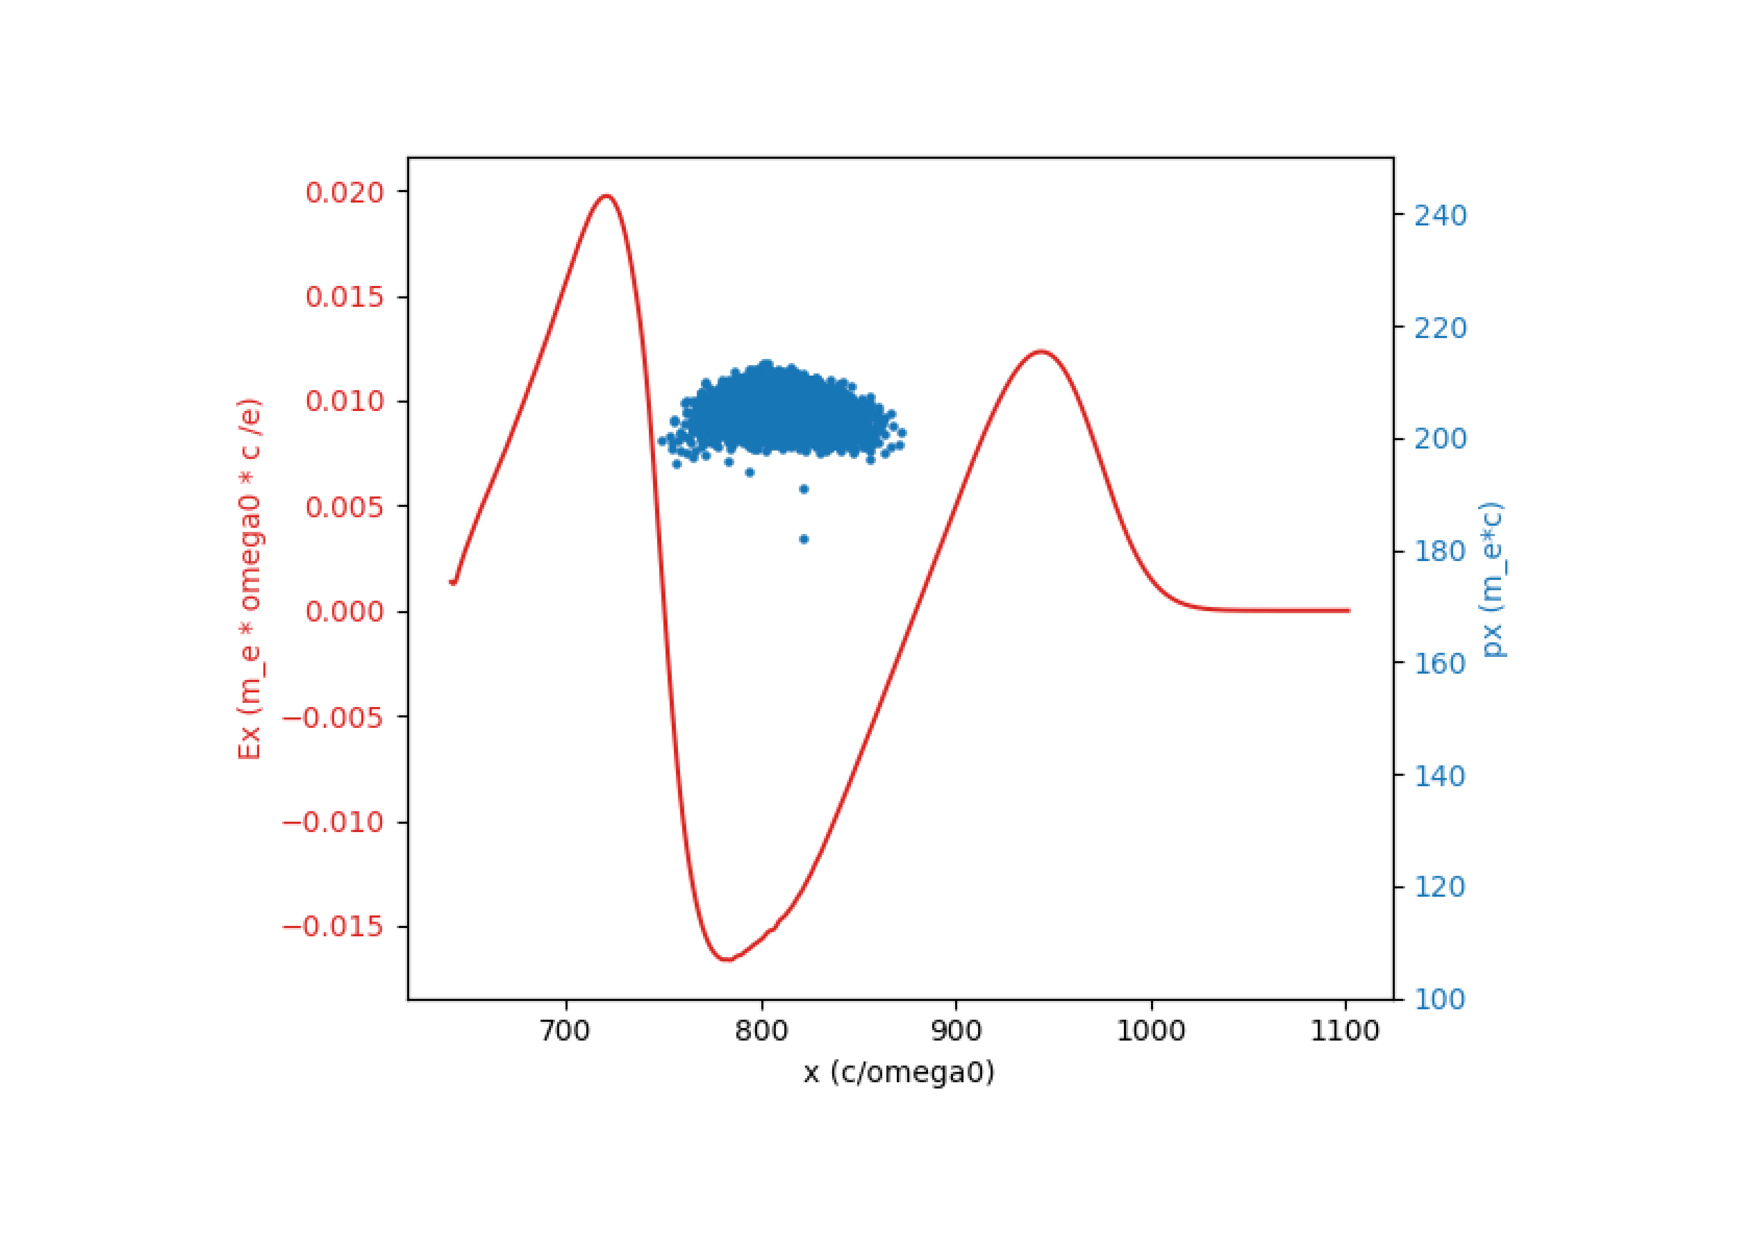
\includegraphics[width=1\linewidth]{ExScatterXPx.pdf}
     \caption{Longitudinal electric field \commandline{Ex} on axis and scatter plot of the bunch electrons' \commandline{x} and \commandline{px}, at iteration \commandline{1000}. }\label{ExScatterXPx}
   \end{minipage}\hfill
   \begin{minipage}{0.48\textwidth}
     \centering
     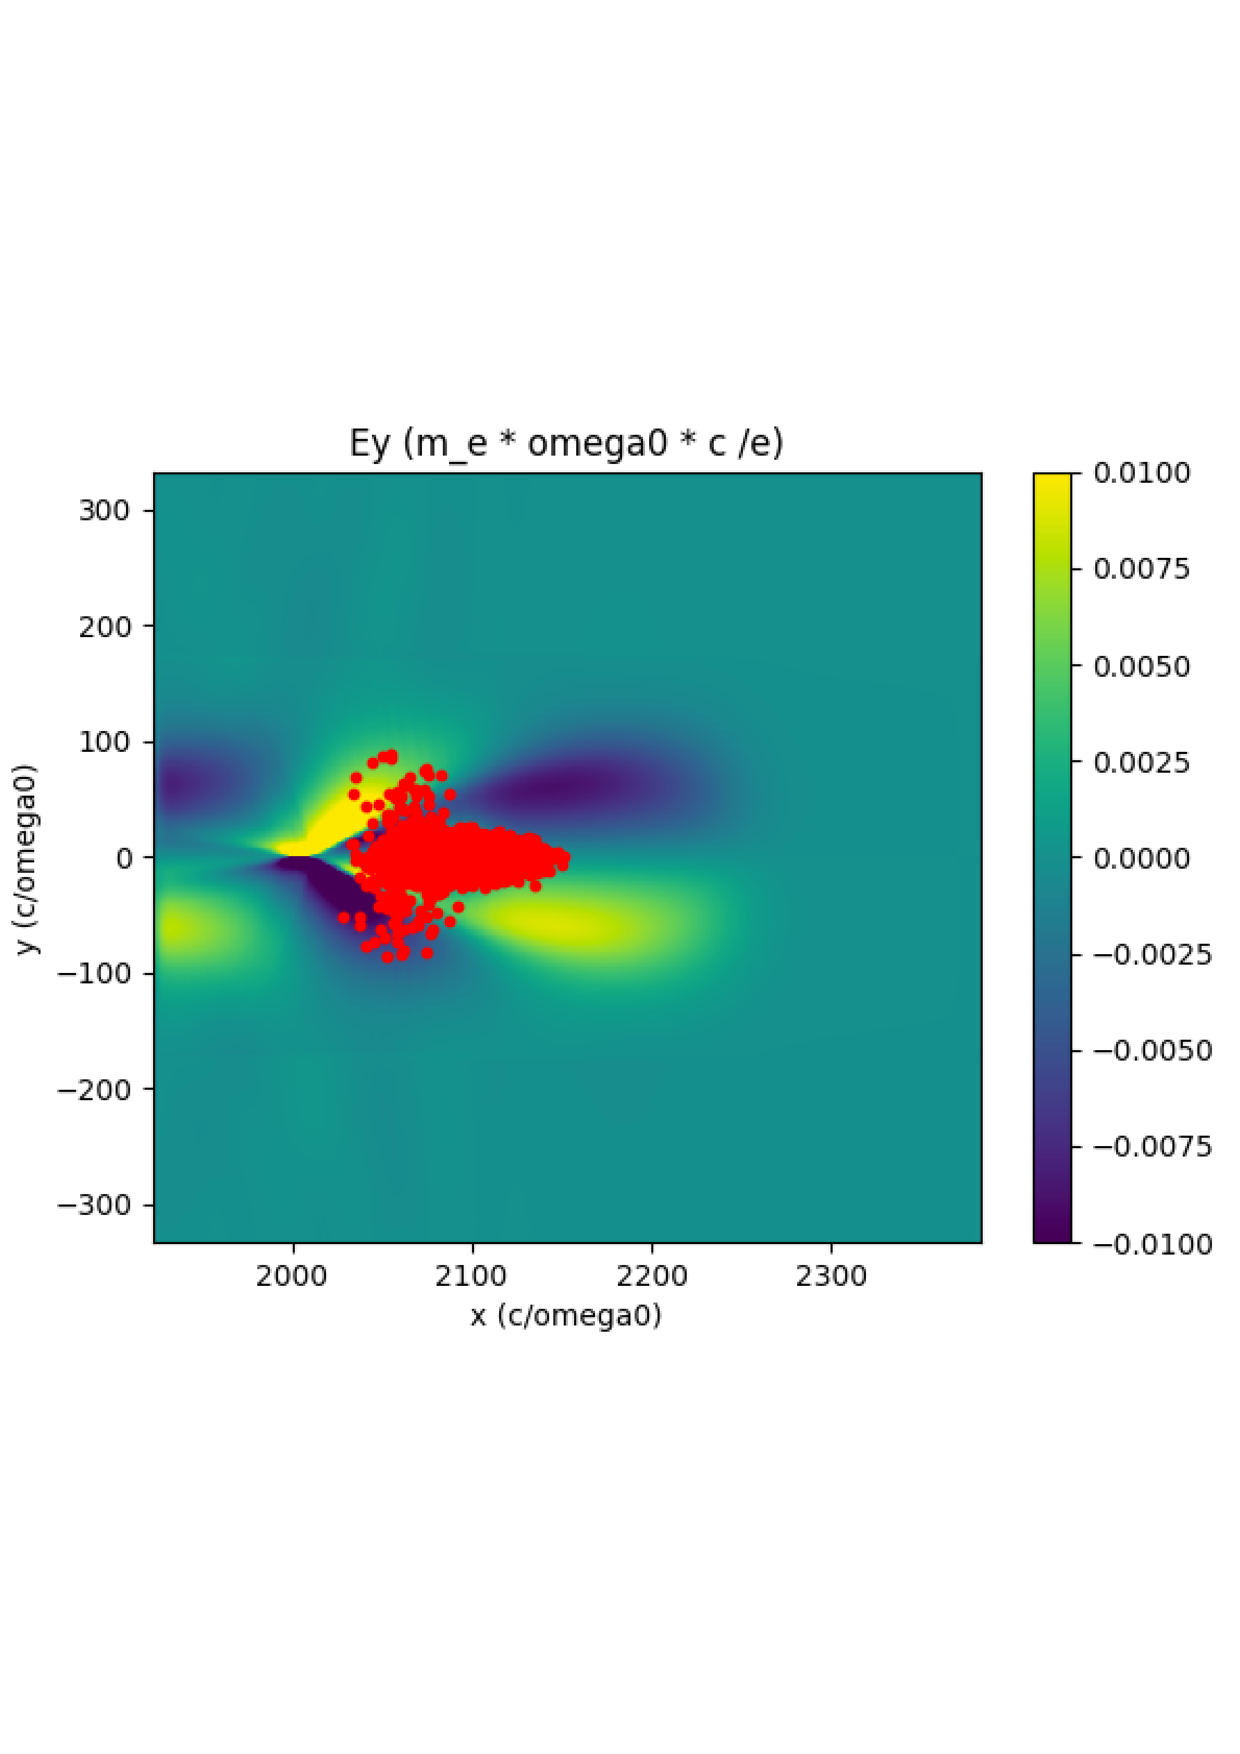
\includegraphics[width=1\linewidth]{EyScatterXY.pdf}
     \caption{Electric field \commandline{Ey} on the plane $xy$ and scatter plot of the bunch electrons' \commandline{x} and \commandline{y} coordinates, at iteration \commandline{3000}. }\label{EyScatterXY}
   \end{minipage}
\end{figure}


\appendix

\begin{appendices}
\section{Crash course on the \commandline{happi} postprocessing library}\label{happi}
A fundamental part of working with simulation codes is of course the postprocessing of the results. \smilei includes an entire library for postprocessing based on Python. However, to  plot your first results and make quantitative evaluations you don't need to be an expert of this language.

For your convenience and quick reference, here we include only the commands you will need for this practical. Do not hesitate to copy and paste the following commands in \commandline{IPython} and adapt them to the problem you are solving.

Remember that the results are in normalized units. The library \commandline{happi} also allows to convert to SI units, but this will not be taught in this practical (details in the documentation online \url{https://smileipic.github.io/Smilei/post-processing.html}).

\subsection*{Compilation of \commandline{happi}}
It is sufficient to use the command \commandline{make happi} in the code folder (after you have loaded the Python modules, see the file \commandline{RucheEnvironment.pdf}). Then, to analyze the results of your simulation, open the \commandline{IPython} interface (just use the command \commandline{ipython} in the command line terminal). 

\subsection*{Open a simulation}
To import the library \commandline{happi} in \commandline{IPython} and open a simulation in the folder,  called for example \commandline{"path/to/simulation"}, use:\\

\commandline{import happi; S =  happi.Open("path/to/simulation")}\\

This will create an object called \commandline{S}, our simulation, which contains all the necessary data, taken from the input namelist and from the output files. You can easily access parameters from the input namelist, for  example:\\

\commandline{S.namelist.dx}

\commandline{S.namelist.Main.geometry}\\

In general, if you tap \commandline{S.} or adding the name  of the blocks and then using the tab key, you will see the available blocks and variables.

\subsection*{Plot diagnostics}
To open a specific diagnostic, like the \commandline{Probe1} defined in the namelist, and plot the longitudinal electric field \commandline{Ex} contained in that diagnostic, use:\\

\commandline{S.Probe.Probe1("Ex").plot()}\\

Other physical fields defined on the grid that you can plot are for example  \commandline{Ey},  \commandline{Rho} (the charge density). Remember  that you can also specify operations on the fields, like \commandline{2.*Ey-Ex}, when you declare your variable.

By default, the last command will only plot the requested field obtained in the last simulation output available for that diagnostic. You may instead be interested in a specific iteration of the simulation (in code  units), like iteration $1200$. To plot only that timestep, just specify it inside the diagnostic block:\\

\commandline{S.Probe.Probe1("Ex", timesteps=1200).plot()}\\

Remember that this timestep corresponds to physical time $1200*\rm{dt}$, where $\rm{dt}$ is the simulation timestep,  which can be found with \commandline{dt=S.namelist.Main.timestep}.

To know which iterations are available for your diagnostic, you can use:\\

\commandline{S.Probe.Probe1("Ex").getAvailableTimesteps()}

\subsection*{Visualize multiple timesteps}
Normally you will have a sequence of outputs, so you may want to see an animation of the outputs or to be able to slide between the saved timesteps. It is possible to do it with these commands respectively:\\

\commandline{S.Probe.Probe1("Ex").animate()}

\commandline{S.Probe.Probe1("Ex").slide()}

In the last case, just slide with the horizontal bar to see the evolution of the plotted quantity at different iterations.

\subsection*{Modify elements to the plot}
Like in Python, you may be interested into specifying the figure number, or change the colormap, or specifying a maximum or minimum value plotted. You can include the same corresponding keywords inside the plot/animate/slide command. As an example where all these elements are specified:\\

\commandline{S.Probe.Probe1("Ex").plot( figure=2, vmin = -0.01, vmax  = 0.01 , cmap = "seismic")}

\subsection*{Plot multiple lines}
You may be interested in visualizing multiple curves in the same plot window. The command \commandline{happi.multiPlot} is what you need.\\

For example, if you want to plot two quantities from the same simulation, scaling them through multiplying factors:\\

\commandline{import happi; S =  happi.Open("path/to/simulation")}

\commandline{E = S.Probe.Probe1("0.1*Ex", timesteps=1000, label = "E")}

\commandline{rho = S.Probe.Probe1("-10.*Rho", timesteps=1000, label="charge density")}

\commandline{happi.multiPlot(E, rho, figure = 1)}\\

The previous example draws two  curves, but you can use \commandline{multiPlot} to plot more curves.

Note that you can plot also different timesteps from the same simulation with the same procedure. 

Similarly, you can plot two quantities from two or more  simulations:\\

\commandline{import happi}

\commandline{S1 = happi.Open("path/to/simulation1"); Ex1 = S1.Probe.Probe0("Ex",timesteps=1000)}

\commandline{S2 = happi.Open("path/to/simulation2"); Ex2 = S2.Probe.Probe0("Ex",timesteps=1000)}

\commandline{happi.multiPlot(Ex1,Ex2)}

\subsection*{Export the data}
Those shown above are all the \commandline{happi} commands you may need for this practical. If you prefer instead to analyze your results with \commandline{numpy} arrays in Python, you can easily export your diagnostic to a \commandline{numpy} array, for example:\\

\commandline{import happi; import numpy as np}

\commandline{S =  happi.Open("path/to/simulation")}

\commandline{myArrayVariable = S.Probe.Probe1("Ex").getData()} 

\commandline{myArrayVariable = S.Probe.Probe1("Ex", timesteps=1200).getData()}

\commandline{myArrayVariable = np.asarray(myArrayVariable) }\\

In case you want to export the data to a text file \commandline{.txt} and read it with another language, you can write this array on a text file using:\\

\commandline{np.savetxt("file\_name.txt", myArrayVariable)}

\section{Why working with normalized units?}\label{normalized units}

Interfacing with the real world is surely easier with SI units, nonetheless simulation codes  work with normalized units. The normalization depends on the characteristic scales of the problem, so using normalized units has two main advantages:
\begin{itemize}
\item If you work with numbers near to 1, you are less prone to machine precision errors. For example, imagine to describe the spatial scales of molecules with chilometers, using 8 bits (1 byte). Your byte will not be able to keep  the necessary precision. For this reason it is always recommended (and often necessary) to rescale your quantities with the scales of interest (e.g. in our case the velocities by the speed of light and so on);
\item Once you perform a simulation with a certain number of normalized quantities, you can use your results for an infinite number of real-life experiments, you just need to rescale properly and coherently all your results. This provided that the physical equations involved do not change at the chosen scales.
\end{itemize}




\end{appendices}

\bibliographystyle{plain}
\bibliography{references}




 


\end{document}

